%============================================================
%  results.tex  –  Chapter 6
%============================================================
\chapter{Results}
\label{ch:results}

In this chapter, the results of the OVOS implementation are presented and analysed. The content is structured into several sections, each reflecting a key aspect of the results. The main OVOS results are presented in Section~\ref{sec:results_ovos}, reflecting on effect of the number of active virtual orbitals, initialisation strategy, and basis set choice. Next, the performance of OVOS orbitals as a VQE reference state is presented in Section~\ref{sec:results_vqe}, where we comment on convergence behaviour and energy recovery, and how well the OVOS orbitals capture Brueckner orbitals. Finally, it is reflected on if we allow orbital optimization in VQE, how the OVOS orbitals perform as a starting point for orbital optimization in VQE, and if they can help to reach better minima in the orbital optimization landscape.

% ---------------------------------------------------------------
% WRITING TIPS – RESULTS
% ---------------------------------------------------------------
% Goal: Present your data clearly and objectively.
%       DESCRIBE the data – do not interpret or explain yet
%       (that belongs in Discussion, which here is folded into
%       Results or a combined Results & Discussion chapter), 
%       there is no separate Discussion chapter in this thesis.
%       At MSc level, integrating discussion into results is fine.
%
% Suggested sections and content:
%
%  6.1  Validation Against Reference Values
%       - Compare your full-space MP2 energies with PySCF's built-in
%         MP2 and with the values quoted in Adamowicz & Bartlett Table I.
%       - This validates your implementation before presenting OVOS data.
%       - A table: molecule | basis | E_corr(PySCF MP2) |
%         E_corr(your code) | deviation?
%
%  6.2  Energy Recovery as a Function of Active Virtual Orbital Count
%       - This is your main result.
%       - For each molecule and at least two basis sets:
%         plot η = E_corr(OVOS) / E_corr(full) vs. N_virt/N_virt^max.
%       - Expected: S-shaped curve rising steeply, reaching ~90% at 50%.
%       - Use the data in branch/data/ to generate these plots.
%       - Consider a composite figure (one panel per molecule).
%       - Reference Adamowicz & Bartlett's numbers for CH₂ if available.
%
%  6.3  Convergence Behaviour
%       - Show convergence of E_corr vs. iteration number for a
%         representative case (e.g., H₂O/cc-pVDZ, N=8 virtual orbs).
%       - Highlight oscillations if present and explain briefly.
%       - Provide iteration count tables: molecule | basis | N_virt |
%         iterations to convergence.
%
%  6.4  Effect of Initialisation Strategy
%       - Compare "RHF", "prev", and "random" initialisation for the
%         same molecule/basis set.
%       - Table or plot showing final E_corr and iterations for each.
%       - Does random sampling find a better minimum? For which cases?
%
%  6.5  Basis Set Dependence
%       - Compare energy recovery curves across basis sets for one molecule
%         (e.g., CH₂: 6-31G, cc-pVDZ, cc-pVTZ).
%       - Does a larger basis set require more virtual orbitals to
%         achieve the same recovery fraction?
%
%  6.6  Comparison with Adamowicz & Bartlett (1987)
%       - Direct comparison for CH₂ (their published test case).
%       - Discuss any differences: UHF vs. RHF reference, basis set.
%
%  6.7  Computational Cost
%       - Wall-clock time vs. N_virt (from profiling data in branch/profil/).
%       - Identify the bottleneck step (Hessian assembly, integral transform).
%       - Scaling analysis: compare empirical scaling to theoretical O(N⁶).
%
% Tips:
%   - Every plot needs: axis labels (with units!), legend, clear caption.
%   - Every table needs: caption above, footnotes for symbols/abbreviations.
%   - Show error bars only if you have statistical data (random sampling).
%   - Use consistent colour scheme across all figures.
%   - Refer to EVERY figure and table in the text before it appears.
%   - Do not bury the lead – the energy recovery plot is the centrepiece.
%
% Plotting: use the data from branch/data/ with Python/Matplotlib.
%   Place exported .pdf or .pgf figures in figures/.
% ---------------------------------------------------------------


\section{OVOS}
\label{sec:results_ovos}

This section presents the MP2 correlation energy recovered as a function of the number of active virtual orbitals for each test molecule and basis set. The results are presented for all test molecules in the cc--pVDZ basis. The convergence behaviour of the OVOS algorithm is also analysed, with a focus on cases where convergence issues arise. The effect of different initialisation strategies on the convergence and energy recovery is explored. Lastly, the c--pVDZ results are compared against the 6--31G results to assess the basis set dependence of the OVOS algorithm.

\subsection{correlation energy of OVOS}
\label{subsec:results_ovos_mp2}
% ---------------------------------------------------------------
% [SECTION INTRO – 6.2]
%   "This section presents the central result of the thesis: the fraction
%    of the full-space MP2 correlation energy, $\eta = E_{\rm corr}^{\rm OVOS}/
%    E_{\rm corr}^{\rm MP2}$, recovered as a function of the ratio
%    $N'_{\rm act.unocc}/N_{\rm act.unocc}$ for each test molecule and basis set."
%
% [WHAT TO COVER]
%   - Report $\eta$ curves for all 9 molecules at 6-31G and cc-pVDZ.
%   - Expected pattern: rapid initial rise, approaching 1 as $N' \to N_{\rm act.unocc}$.
%   - Compare against Adamowicz \& Bartlett's claim of $\eta \approx 0.9$ at $N'=N/2$.
%   - Discuss the ``best'' and ``worst'' systems (which benefit most?).
%   - Use the data in \texttt{branch/data/} for all plots.
%
% [FIGURE – MAIN RESULT]
%   x-axis: $N'_{\rm act.unocc}/N_{\rm act.unocc}$ (fraction, 0 to 1)
%   y-axis: $\eta = E_{\rm corr}^{\rm OVOS}/E_{\rm corr}^{\rm MP2}$ (0 to 1)
%   One curve per molecule; one panel per basis set (or combined).
%   Add horizontal dashed line at $\eta = 0.9$.
%   Caption: ``Energy recovery fraction $\eta$ as a function of the
%   active virtual orbital fraction for all test molecules in the
%   [basis] basis. The dashed line marks 90\% recovery.''
%   Export as \texttt{figures/fig\_eta\_recovery.pdf}.
%
% [FIGURE – COMPOSITE PANEL (optional)]
%   $3 \times 3$ subplot grid, one molecule per panel, coloured by basis set.
%   Caption: ``Energy recovery curves for all nine test molecules.
%   Each panel shows three basis sets: 6-31G (blue), cc-pVDZ (orange),
%   cc-pVTZ (green).'' Export as \texttt{figures/fig\_eta\_all.pdf}.
%
% [LEAD-IN TO §6.3]
%   "The rate of convergence of each OVOS run to its final energy
%    is quantified in the following section."
% ---------------------------------------------------------------

The results of the OVOS algorithm for all test molecules in the cc--pVDZ basis sets for start guess RHF, previous, and random are presented in this section. We explore the results of the correlation energy recovered by OVOS as a function of the number of active unoccupied orbitals $N'_{\rm act.unocc}$.  


% As the OVOS algorithm optimises the orbitals to recover correlation energy, the choice of initial orbitals can influence the convergence path and final energy. In this section, I compare three initialisation strategies: default SCF (RHF), warm-start from a previous $N'$ run, and random unitary sampling. For the random sampling, I generate 1000 random unitary transformations of the initial orbitals and run OVOS for each, recording the final correlation energy. The best result from the random sampling is then compared to the default and warm-start strategies. The results for the benchmark molecules in the cc--pVDZ basis are presented below. 



\subsubsection*{CO}

We observe that OVOS nearly steadily recovers increasingly more of the total correlation energy $E_{\rm corr}^{\rm OVOS}$ as $N'_{\rm act.unocc}$ increases, with the percentage of correlation energy recovered reaching 100\% at full space $N'_{\rm act.unocc} = 21$ for start guess RHF. Reaching 90\% recovery at $N'_{\rm act.unocc} = 13$ for all start guesses, which is approximately 62\% of the total number of active unoccupied orbitals for previous start guess. The OVOS algorithm results for $CO$ in the cc--pVDZ basis through each $N'_{\rm act.unocc}$ to full space of active unoccupied orbitals for the three start guesses are shown in Figure~\ref{fig:CO_cc-pVDZ_ovos}.

We mark the difference the OVOS algorithm make, amount of correlation energy recovered, at each $N'_{\rm act.unocc}$ by an initial point with iterations to the final point for each $N'_{\rm act.unocc}$ in Figure~\ref{fig:CO_cc-pVDZ_ovos} as the points for each $N'_{\rm act.unocc}$. The most recovered correlation energy is between $N'_{\rm act.unocc} = 3$ and $N'_{\rm act.unocc} = 10$ with $\Delta E_{\rm corr}^{\rm OVOS} \simeq 0.1$ Hartree for start guess RHF. It is observed that start guess random consistently finds higher initial correlation energies, and oppositely start guess previous finds consistently lower correlation energies. It is observed that the change in converged correlation energy from previous number of active unoccupied orbitals falls as $N'_{\rm act.unocc}$ increases, with a few exceptions like between $N'_{\rm act.unocc} = 4$ and $N'_{\rm act.unocc} = 5$. Convergence is nearly achieved in all cases, only $N'_{\rm act.unocc} = 6$ for RHF reaches maximum iterations and is non convergened, see Appendix~\ref{appb:CO_cc-pVDZ_ovos_6_iterations}. Iteration counts show no clear pattern for any of the start guesses as $N'_{\rm act.unocc}$ reaches the total number of active unoccupied orbitals. The correlation energy iterations are plotted in Appendix~\ref{appb:CO_cc-pVDZ_ovos_iterations} to show the convergence behaviour of the OVOS algorithm for CO in the cc--pVDZ basis at each $N'_{\rm act.unocc}$.

Shortcomings of the OVOS algorithm are observed at $N'_{\rm act.unocc} = 11$ through to $N'_{\rm act.unocc} = 17$ for the different start guesses, where the algorithm fails to converge at an agreeable correlation energy, and instead converges to a local minimum with a much higher correlation energy. It is however observed in this interval that RHF performs more similar to the trend of other numbers of active unoccupied orbitals. This suggests that the orbital optimization landscape in OVOS has multiple local minima, which can trap the algorithm if the initial guess is not close enough to the global minimum. This is backed up by the fact it was observed that the Hessian matrix has negative eigenvalues in these regions, as the blocks within grow in size, capturing more of the off-diagonal elements.

\begin{figure}[H]
    \centering
    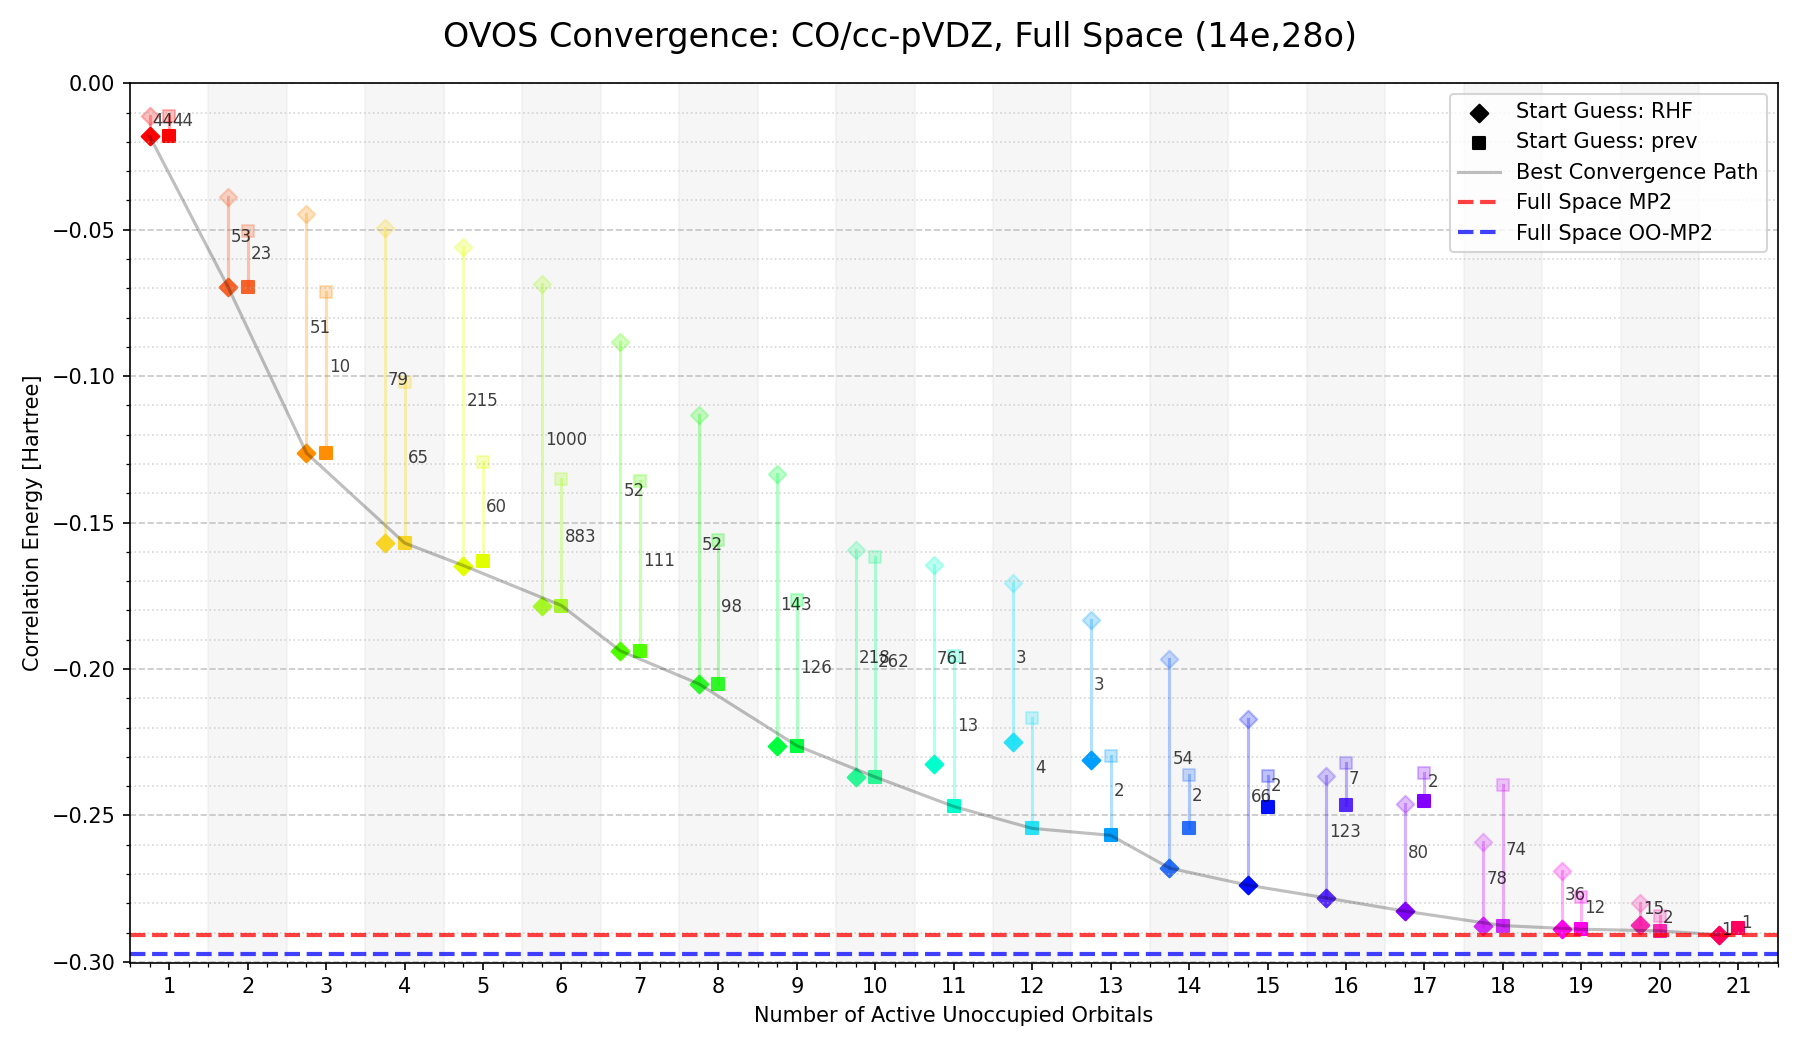
\includegraphics[width=0.9\textwidth]{figures/OVOS_PLOTS/CO/cc-pVDZ/ovos_convergence_CO_cc-pVDZ.png}
    \caption{Convergence of the MP2 correlation energy for CO in the cc--pVDZ basis at each $N'_{\rm act.unocc}$. The OVOS algorithm takes RHF as start guess. Dashed red line marks the MP2 correlation energy at full space, PySCF reference. Dashed blue line marks the OOMP2 correlation energy at full space, PySCF reference. A line is drawn to connect the points for visualization purposes, at which the number of iterations to convergence is annotated.}
    \label{fig:CO_cc-pVDZ_ovos}
\end{figure}

\newpage

\subsubsection*{H2O}

OVOS recovers increasingly more of the total correlation energy $E_{\rm corr}^{\rm OVOS}$ as $N'_{\rm act.unocc}$ increases, with the percentage of correlation energy recovered reaching 100\% at $N'_{\rm act.unocc} = 19$ for start guess RHF. Reaching 90\% recovery at $N'_{\rm act.unocc} = 13$, which is approximately 68\% of the total number of active unoccupied orbitals. It is seen that from $N'_{\rm act.unocc} = 17$ the start guesses approximates the full-space correlation energy more closely. The OVOS algorithm results for $H_2O$ in the cc--pVDZ basis through each $N'_{\rm act.unocc}$ to full space of active unoccupied orbitals are shown in Figure~\ref{fig:H2O_cc-pVDZ_ovos}. 

The difference OVOS makes for $H_2O$ at each $N'_{\rm act.unocc}$ is marked in Figure~\ref{fig:H2O_cc-pVDZ_ovos}. The most recovered correlation energy is for $N'_{\rm act.unocc} \in \{3, 4, 9, 10\}$ with $\Delta E_{\rm corr}^{\rm OVOS} \simeq 0.1$ Hartree for start guess RHF. Likewise for $CO$ it is observed start guess previous finds consistently lower correlation energies, and start guess random finds consistently higher correlation energies. Convergence is achieved in nearly all cases, except three cases for $N'_{\rm act.unocc} = 13$ for RHF, and $N'_{\rm act.unocc} = 12, 8$ for previous, which is observed to agree with the values for the other start guesses, as seen in Figure~\ref{fig:H2O_cc-pVDZ_ovos}. There is no region of non-convergence to a local minimum as $N'_{\rm act.unocc}$ increases like seen for $CO$. Except for a little deviation for $N'_{\rm act.unocc} = 11$ for previous. Iteration counts show no clear pattern as $N'_{\rm act.unocc}$ increases nor between the start guesses, with the highest iteration count at $N'_{\rm act.unocc} = 13$ for random only accounting for converged cases. The correlation energy iterations are plotted in Appendix~\ref{appb:H2O_cc-pVDZ_ovos_iterations} to show the convergence behaviour of the OVOS algorithm for H2O in the cc--pVDZ basis at each $N'_{\rm act.unocc}$.
 
\begin{figure}[H]
    \centering
    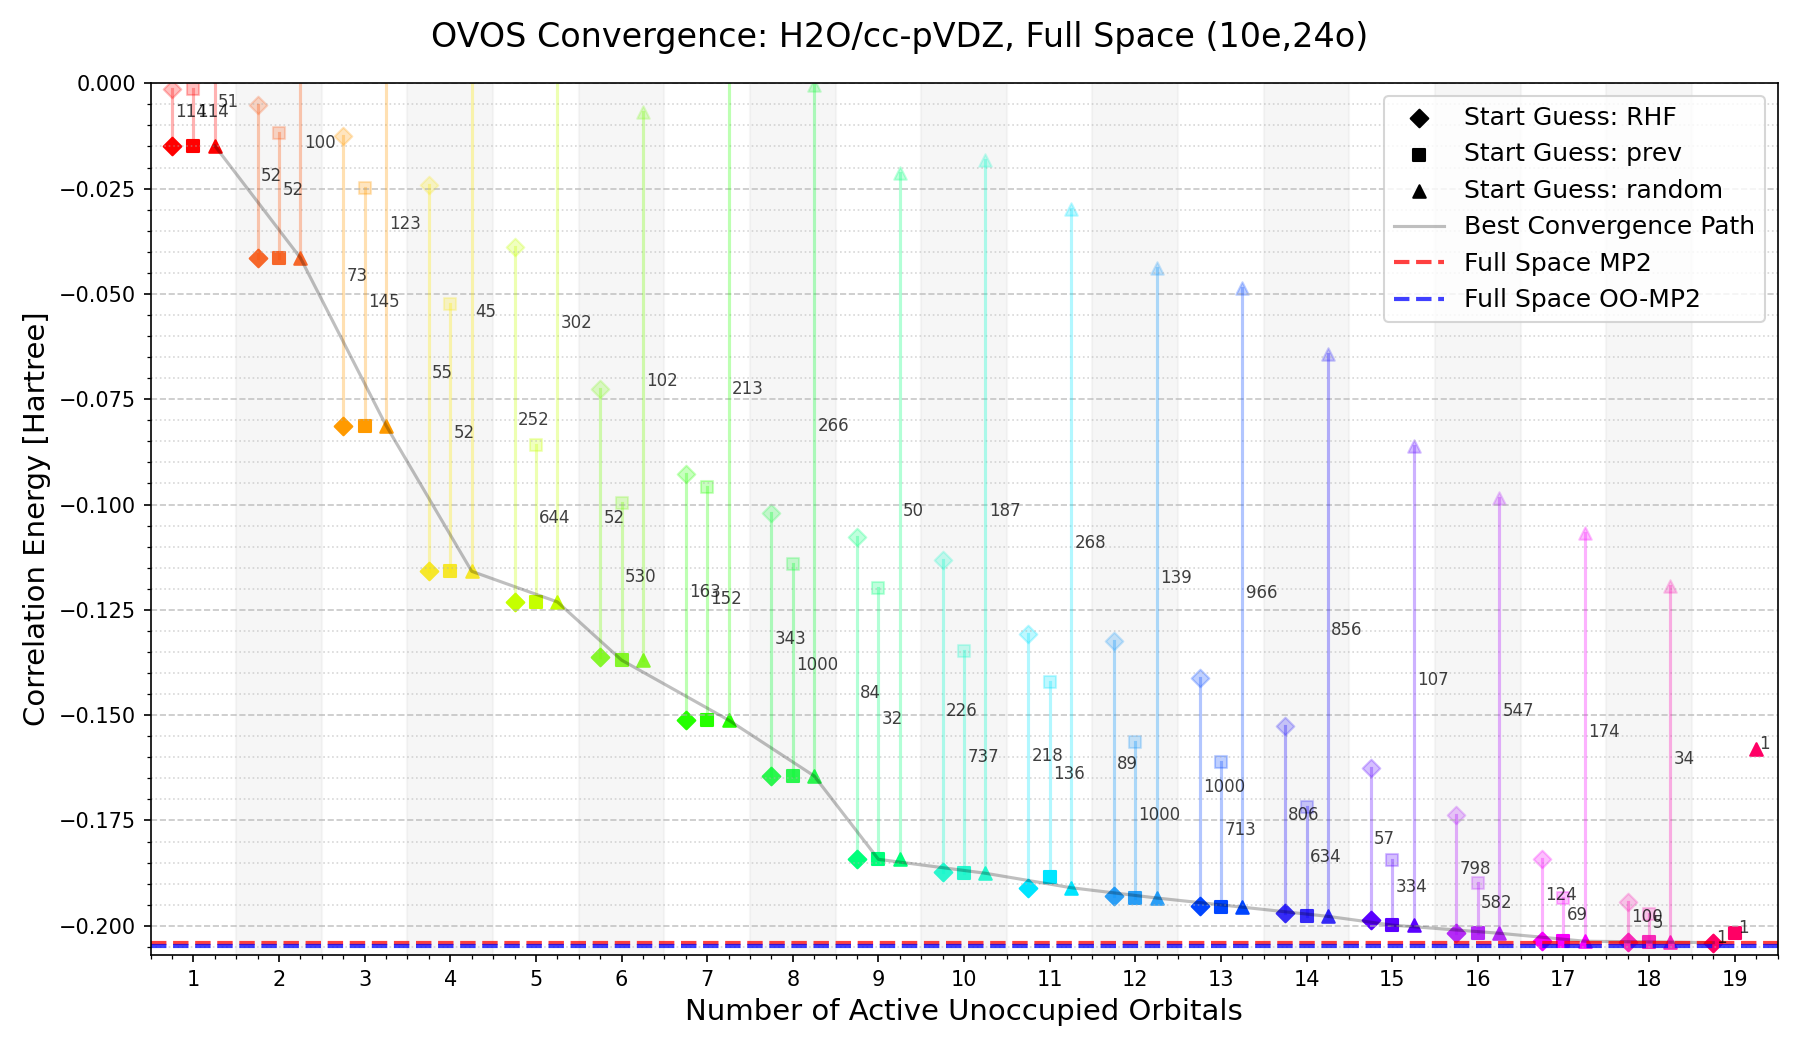
\includegraphics[width=0.9\textwidth]{figures//OVOS_PLOTS/H2O/cc-pVDZ/ovos_convergence_H2O_cc-pVDZ.png}
    \caption{Convergence of the MP2 correlation energy for H2O in the cc--pVDZ basis at each $N'_{\rm act.unocc}$. The OVOS algorithm takes RHF as start guess. Dashed red line marks the MP2 correlation energy at full space, PySCF reference. Dashed blue line marks the OOMP2 correlation energy at full space, PySCF reference. A line is drawn to connect the points for visualization purposes, at which the number of iterations to convergence is annotated.}
    \label{fig:H2O_cc-pVDZ_ovos}
\end{figure}

\newpage

\subsubsection*{HF}

OVOS recovers increasingly more of the total correlation energy $E_{\rm corr}^{\rm OVOS}$ as $N'_{\rm act.unocc}$ increases, with the percentage of correlation energy recovered reaching 100\% at $N'_{\rm act.unocc} = 14$ for RHF. Reaching 90\% recovery at $N'_{\rm act.unocc} = 9$, consistence for all start guesses, which is approximately 64\% of the total number of active unoccupied orbitals. The OVOS algorithm results for HF in the cc--pVDZ basis through each $N'_{\rm act.unocc}$ to full space of active unoccupied orbitals are shown in Figure~\ref{fig:HF_cc-pVDZ_ovos}.     

The most correlation energy recovered by OVOS for HF is at $N'_{\rm act.unocc} = 3,4, 9$ with $\Delta E_{\rm corr}^{\rm OVOS} \simeq 0.625$ Hartree for RHF. Here we notice some previous start guesses find higher initial correlation energies than RHF, while the random start guess consistently finds higher correlation energies. Convergence is achieved in all cases for RHF, with iteration counts increasing and decreasing as $N'_{\rm act.unocc}$ increases. Previous finds it reaches max iterations at $N'_{\rm act.unocc} = 5$ and random at $N'_{\rm act.unocc} = 10, 12, 6$. Iteration counts show no clear pattern as $N'_{\rm act.unocc}$ increases, with the highest iteration count at $N'_{\rm act.unocc} = 6$ for previous reaching $867$, undergoing both oscillations and divergence. The correlation energy iterations are plotted in Appendix~\ref{appb:HF_cc-pVDZ_ovos_iterations} to show the convergence behaviour of the OVOS algorithm for HF in the cc--pVDZ basis at each $N'_{\rm act.unocc}$.


% \begin{table}[H]
%     \centering
%     \begin{tabular}{ccccc}
%         \hline
%         $N'_{\rm act.unocc}$ & $E_{\rm corr}^{\rm OVOS}$ (Hartree) & Percentage & $\Delta E_{\rm corr}^{\rm OVOS}$ (Hartree) & Iterations \\ 
%         \hline
%         1    & -1.84737E-02 & 14.35\%     & -1.52027e-2     & 13        \\
%         2    & -4.39109E-02 & 34.12\%     & -2.91136e-2     & 15        \\
%         3    & -8.74131E-02 & 67.92\%     & -5.39991e-2     & 50        \\
%         4    & -1.24045E-01 & 96.39\%     & -5.49038e-2     & 20        \\
%         5    & -1.28136E-01 & 99.57\%     & -2.49738e-2     & 15        \\
%         6    & -1.28694E-01 & 100.0\%     &                 & 1         \\
%         \hline
%     \end{tabular}
%     \caption{Summary of OVOS results for HF in the 6--31G basis at each $N'_{\rm act.unocc}$.}
%     \label{tab:HF_6-31G_results}
% \end{table}
% The table is plotted in Figure~\ref{fig:HF_6-31G_ovos} to show the convergence behaviour of the OVOS algorithm for HF in the 6--31G basis at each $N'_{\rm act.unocc}$.

\begin{figure}[H]
    \centering
    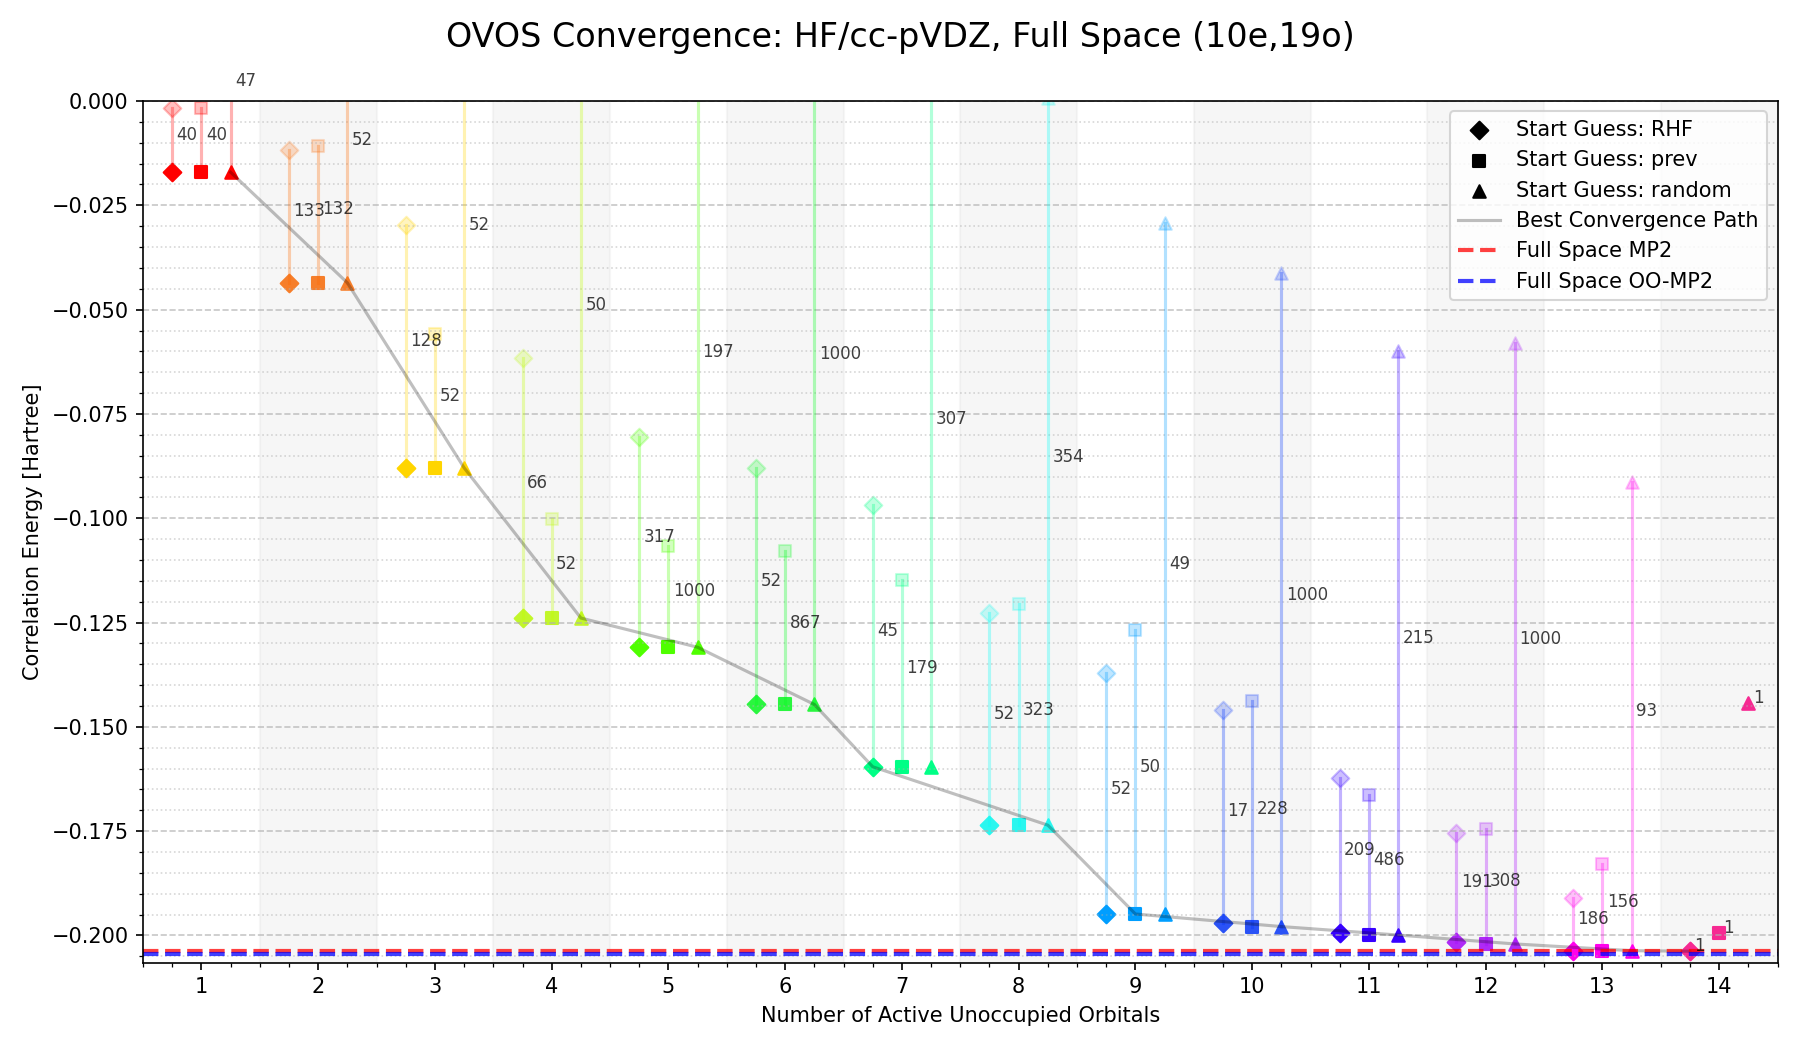
\includegraphics[width=0.9\textwidth]{figures/OVOS_PLOTS/HF/cc-pVDZ/ovos_convergence_HF_cc-pVDZ.png}
    \caption{Convergence of the MP2 correlation energy for HF in the cc--pVDZ basis at each $N'_{\rm act.unocc}$. The OVOS algorithm takes RHF as start guess. Dashed red line marks the MP2 correlation energy at full space, PySCF reference. Dashed blue line marks the OOMP2 correlation energy at full space, PySCF reference. A line is drawn to connect the points for visualization purposes, at which the number of iterations to convergence is annotated.}
    \label{fig:HF_cc-pVDZ_ovos}
\end{figure}


\subsubsection*{NH3}

OVOS recovers increasingly more of the total correlation energy $E_{\rm corr}^{\rm OVOS}$ as $N'_{\rm act.unocc}$ increases, except for $N'_{\rm act.unocc} = 20$ which seems to struggle to the amount that the best of the three start guesses achieves is not lower than the previous $N'_{\rm act.unocc}$. It still holds that the percentage of correlation energy recovered reaches 100\% at $N'_{\rm act.unocc} = 24$ for RHF, and we reach 90\% recovery at $N'_{\rm act.unocc} = 12$ for all start guesses, which is approximately 50\% of the total number of active unoccupied orbitals. It is seen that from $N'_{\rm act.unocc} = 21$ the start guesses approximates the full-space correlation energy more closely. The OVOS algorithm results for NH3 in the cc--pVDZ basis through each $N'_{\rm act.unocc}$ to full space of active unoccupied orbitals are shown in Figure~\ref{fig:NH3_cc-pVDZ_ovos}.

The most correlation energy recovered by OVOS for NH3 is at $N'_{\rm act.unocc} = 3, 4, 5$ with $\Delta E_{\rm corr}^{\rm OVOS} \simeq 0.75$ Hartree for RHF. It is observed previous starts at a lower correlation energy than RHF, oppositely random shows consistent higher initial correlation energies, likewise the previous molecules. At $N'_{\rm act.unocc} = 8$ for RHF and $N'_{\rm act.unocc} = 6, 10$ for previous does OVOS not converge, reaching max iterations, which is observed to stop at an agreeable correlation energy, between $N'_{\rm act.unocc} = 9$ and $N'_{\rm act.unocc} = 10$, as seen in Figure~\ref{fig:NH3_cc-pVDZ_ovos}. Iteration counts show no clear pattern as $N'_{\rm act.unocc}$ increases, with the highest iteration count at $N'_{\rm act.unocc} = 23$ for RHF of $797$, undergoing both oscillations and divergence. The correlation energy iterations are plotted in Appendix~\ref{appb:NH3_cc-pVDZ_ovos_iterations} to show the convergence behaviour of the OVOS algorithm for NH3 in the cc--pVDZ basis at each $N'_{\rm act.unocc}$.

\begin{figure}[H]
    \centering
    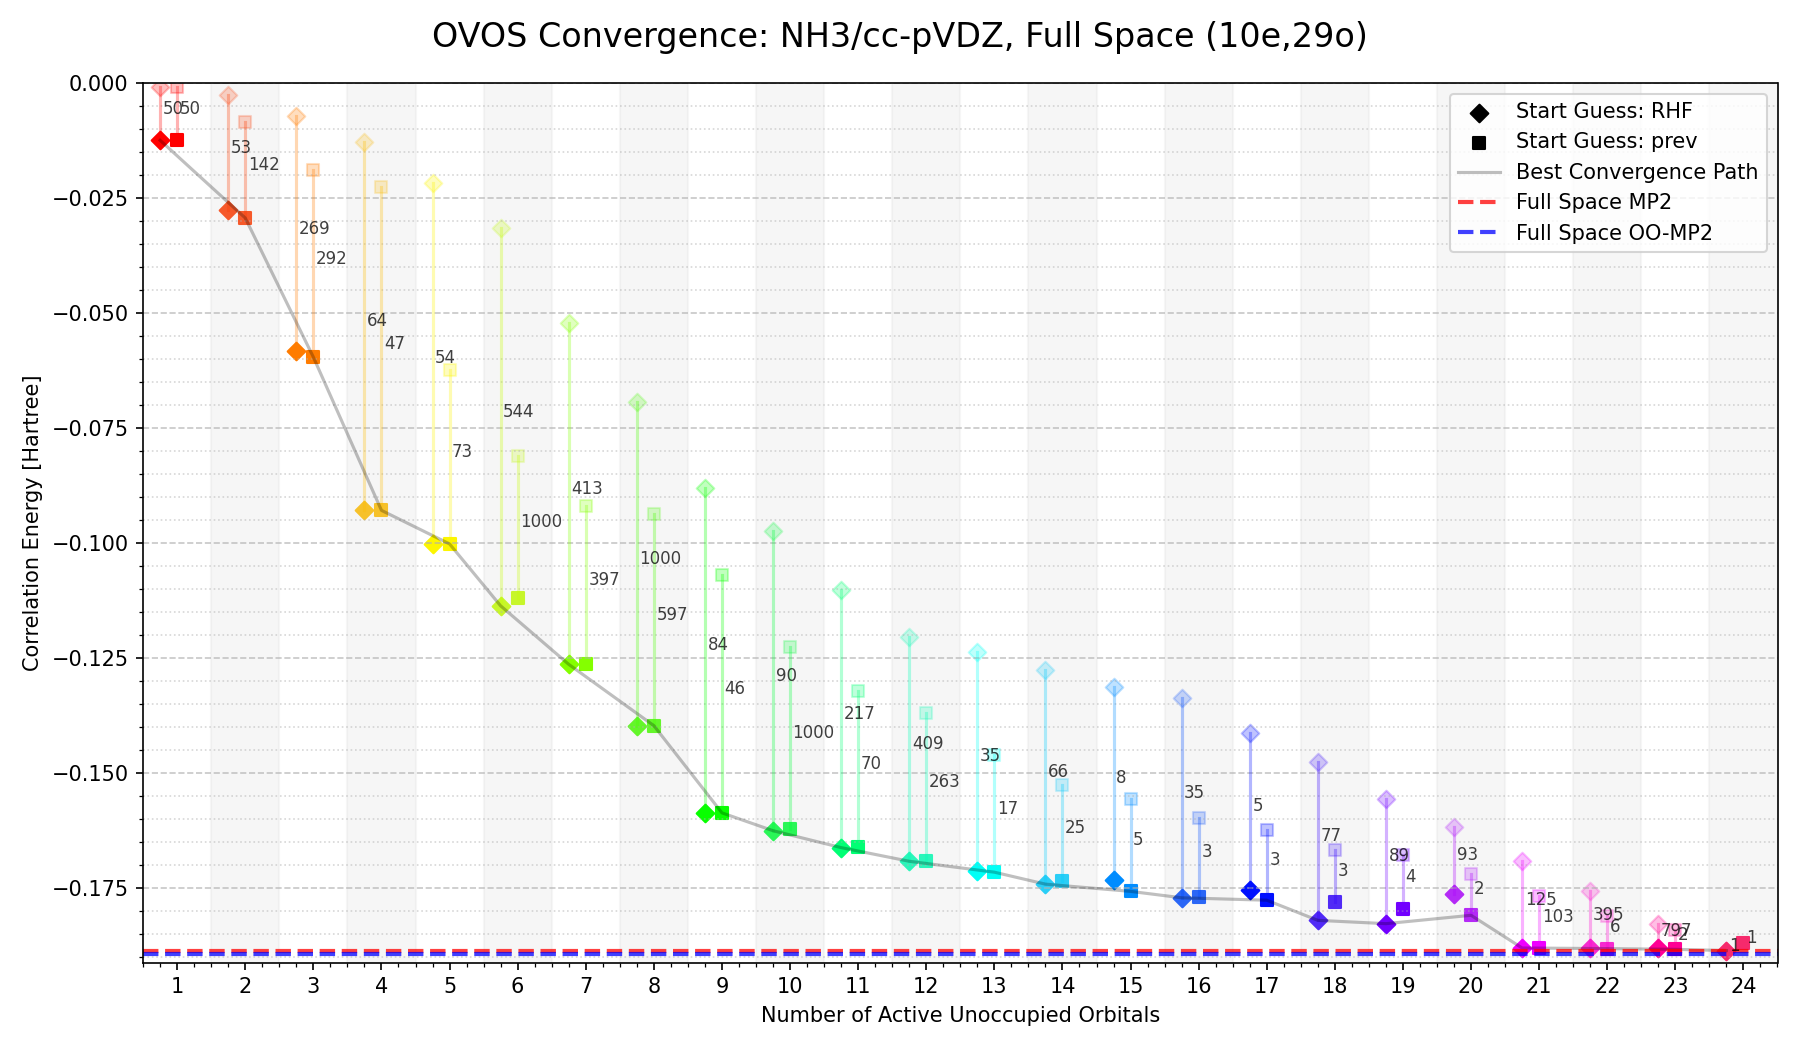
\includegraphics[width=0.9\textwidth]{figures/OVOS_PLOTS/NH3/cc-pVDZ/ovos_convergence_NH3_cc-pVDZ.png}
    \caption{Convergence of the MP2 correlation energy for NH3 in the cc--pVDZ basis at each $N'_{\rm act.unocc}$. The OVOS algorithm takes RHF as start guess. Dashed red line marks the MP2 correlation energy at full space, PySCF reference. Dashed blue line marks the OOMP2 correlation energy at full space, PySCF reference. A line is drawn to connect the points for visualization purposes, at which the number of iterations to convergence is annotated.}
    \label{fig:NH3_cc-pVDZ_ovos}
\end{figure}


\subsubsection*{Li2}

OVOS increasingly recovers more of the total correlation energy $E_{\rm corr}^{\rm OVOS}$ as $N'_{\rm act.unocc}$ increases, quietly slowing down as $N'_{\rm act.unocc}$ approaches $9$, hereafter convergence issues show up at $N'_{\rm act.unocc} = 12$, as multiple points deviates from the expected correlation energy behavior toward full space. The percentage of correlation energy recovered reaches 100\% at $N'_{\rm act.unocc} = 25$ for RHF, and we reach 90\% recovery at $N'_{\rm act.unocc} = 7$, which is approximately 28\% of the total number of active unoccupied orbitals. It is seen that from $N'_{\rm act.unocc} = 22$ the RHF start guess approximates the full-space correlation energy more closely. The OVOS algorithm results for Li2 in the cc--pVDZ basis through each $N'_{\rm act.unocc}$ to full space of active unoccupied orbitals are shown in Figure~\ref{fig:Li2_cc-pVDZ_ovos}. 

The most correlation energy recovered by OVOS for Li2 is at $N'_{\rm act.unocc} = 5,\ 6,\ 7$ with $\Delta E_{\rm corr}^{\rm OVOS} \simeq 0.0125$ Hartree for RHF. Disregarding the convergence issues at higher $N'_{\rm act.unocc}$ values, previous and random show consistent behavior as found for the other molecules. OVOS converges for all $N'_{\rm act.unocc}$, no max iterations show up for any start guess. Iteration counts show no clear pattern as $N'_{\rm act.unocc}$ increases, with the highest iteration count at $N'_{\rm act.unocc} = 23$ of $668$ for random start, undergoing both oscillations and divergence. The region, as seen for $CO$, shows similar bad convergence behavior, here the region is from $N'_{\rm act.unocc} = 12$ to $N'_{\rm act.unocc} = 23$, and only a few points of start guess RHF looks to follow the original trend at $N'_{\rm act.unocc} = 15, 19, 20, 22, 23$. The correlation energy iterations are plotted in Appendix~\ref{app:Li2_cc-pVDZ_ovos_iterations} to show the convergence behaviour of the OVOS algorithm for Li2 in the cc--pVDZ basis at each $N'_{\rm act.unocc}$.

\begin{figure}[H]
    \centering
    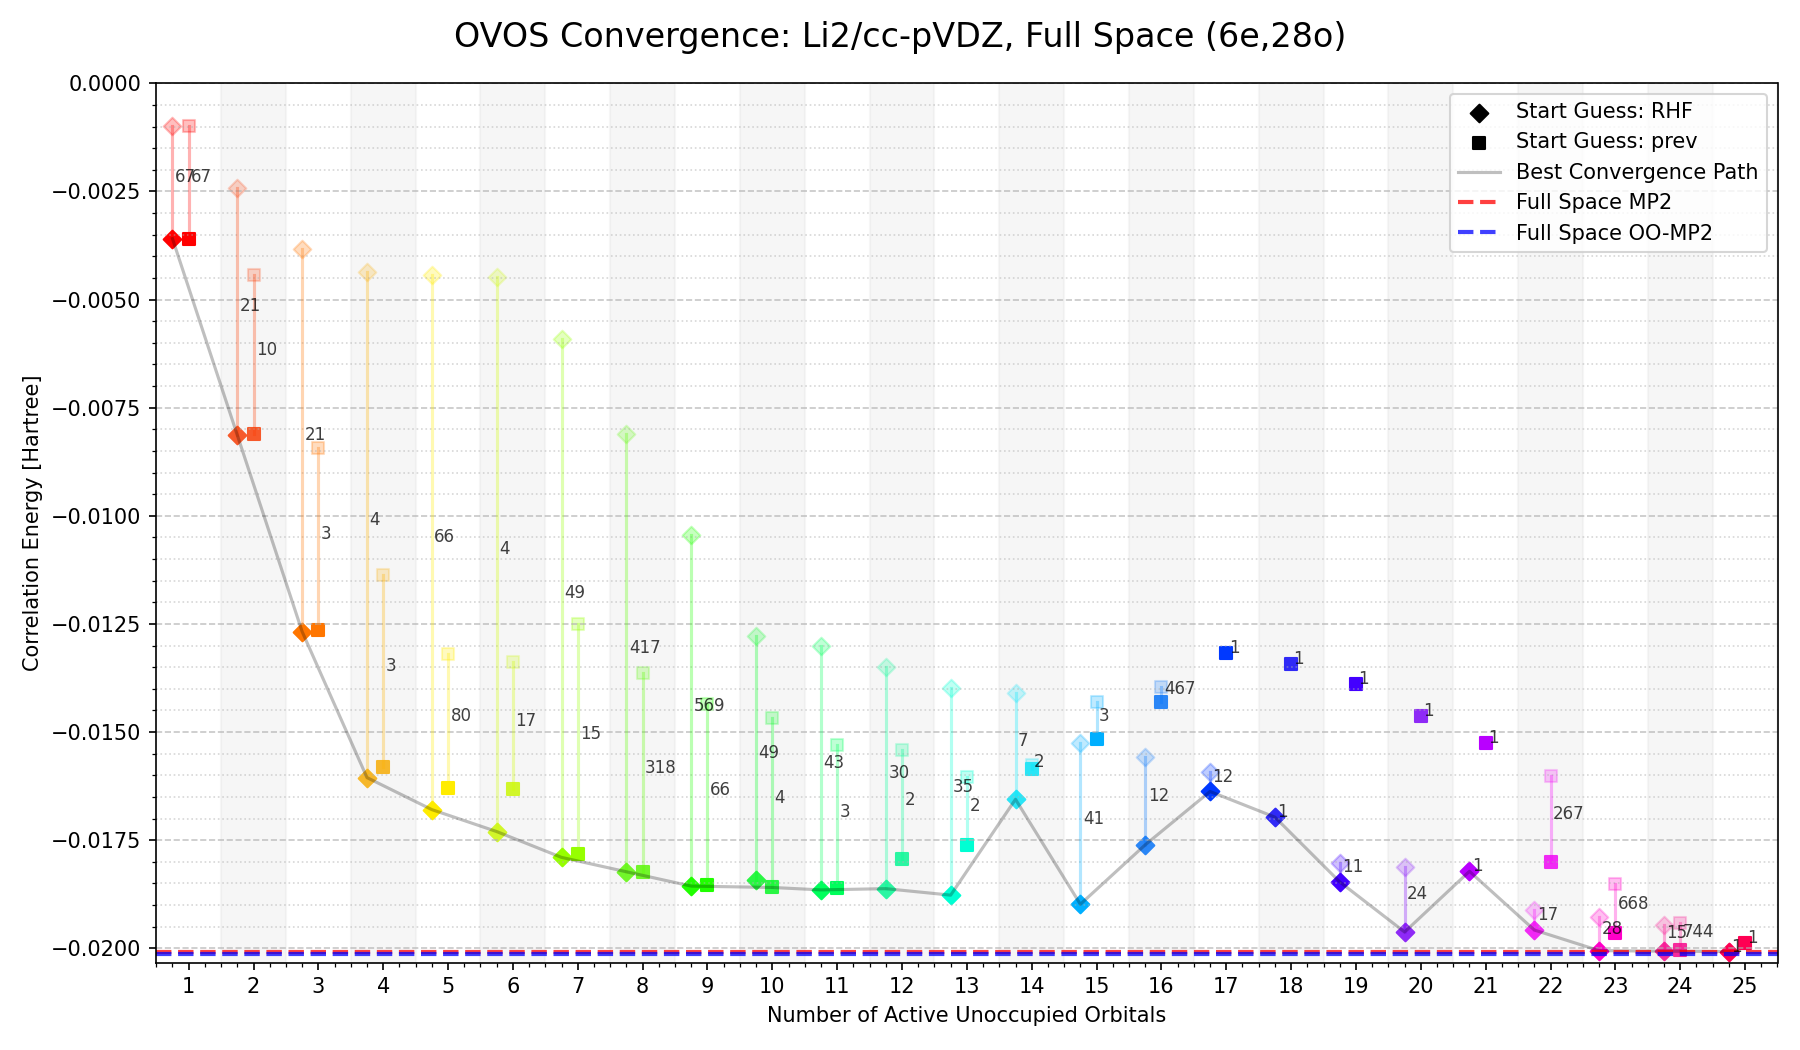
\includegraphics[width=1\textwidth]{figures/OVOS_PLOTS/Li2/cc-pVDZ/ovos_convergence_Li2_cc-pVDZ.png}
    \caption{Convergence of the MP2 correlation energy for Li2 in the cc--pVDZ basis at each $N'_{\rm act.unocc}$. The OVOS algorithm takes RHF as start guess. Dashed red line marks the MP2 correlation energy at full space, PySCF reference. Dashed blue line marks the OOMP2 correlation energy at full space, PySCF reference. A line is drawn to connect the points for visualization purposes, at which the number of iterations to convergence is annotated.}
    \label{fig:Li2_cc-pVDZ_ovos}
\end{figure}




% Just to keep track
% Procentage of total space it took to reach 90\% recovery for each molecule in cc--pVDZ:
% CO: 62\%
% H2O: 68\%
% HF: 64\%
% NH3: 50\%
% Li2: 28\%



% \section{Convergence Behaviour "Skip?"}
% % ---------------------------------------------------------------
% % [SECTION INTRO – 6.3]
% %   "The OVOS convergence behaviour --- the evolution of the MP2
% %    correlation energy per iteration --- reveals the numerical stability
% %    and efficiency of the Newton-Raphson orbital optimisation.
% %    This section presents representative convergence profiles and
% %    summarises iteration counts across the test set."
% %
% % [WHAT TO COVER]
% %   - Convergence means $|\Delta E_{\rm corr}| < 10^{-8}$ achieved.
% %   - Show a representative case, e.g. H\textsubscript{2}O/cc-pVDZ, $N'=8$.
% %   - Discuss cases of slow or oscillatory convergence (large active spaces?)
% %   - Report iteration counts vs.~$N'_{\rm act.unocc}$: do larger spaces need more iterations?
% %
% % [FIGURE]
% %   x-axis: Iteration number | y-axis: $|\Delta E_{\rm corr}|$ (log scale)
% %   Caption: ``Convergence of the MP2 correlation energy for
% %   H\textsubscript{2}O/cc-pVDZ with $N'_{\rm act.unocc} = 8$ active virtual
% %   spin-orbitals. The dashed line marks the convergence threshold $10^{-8}$~$E_h$.''
% %
% % [TABLE]
% %   Columns: Molecule | Basis | $N'_{\rm act.unocc}$ | Iterations | Converged?
% %   Caption: ``Iteration counts to convergence for all OVOS calculations.
% %   Maximum iterations: [value].''
% %
% % [LEAD-IN TO §6.4]
% %   "The degree to which convergence and final energy depend on the
% %    initial orbital guess is investigated in the following section."
% % ---------------------------------------------------------------

% In this section, I present the convergence profiles of the OVOS algorithm for the test molecules in the 6--31G and cc--pVDZ basis sets. 

% Convergence is achieved when $|\Delta E_{\rm corr}| < 10^{-8}$~Hartree for at least 50 consecutive iterations. Some cases, would get stuck in a local minimum achieving convergence. The consecutive iteration criterion then avoids these false positives, and help identify true convergence, a global minimum. For example, ... 

% "illustrate a good example of convergence and a bad example of convergence, with the corresponding plots in the appendix."

% \begin{figure}[ht]
%     \centering
%     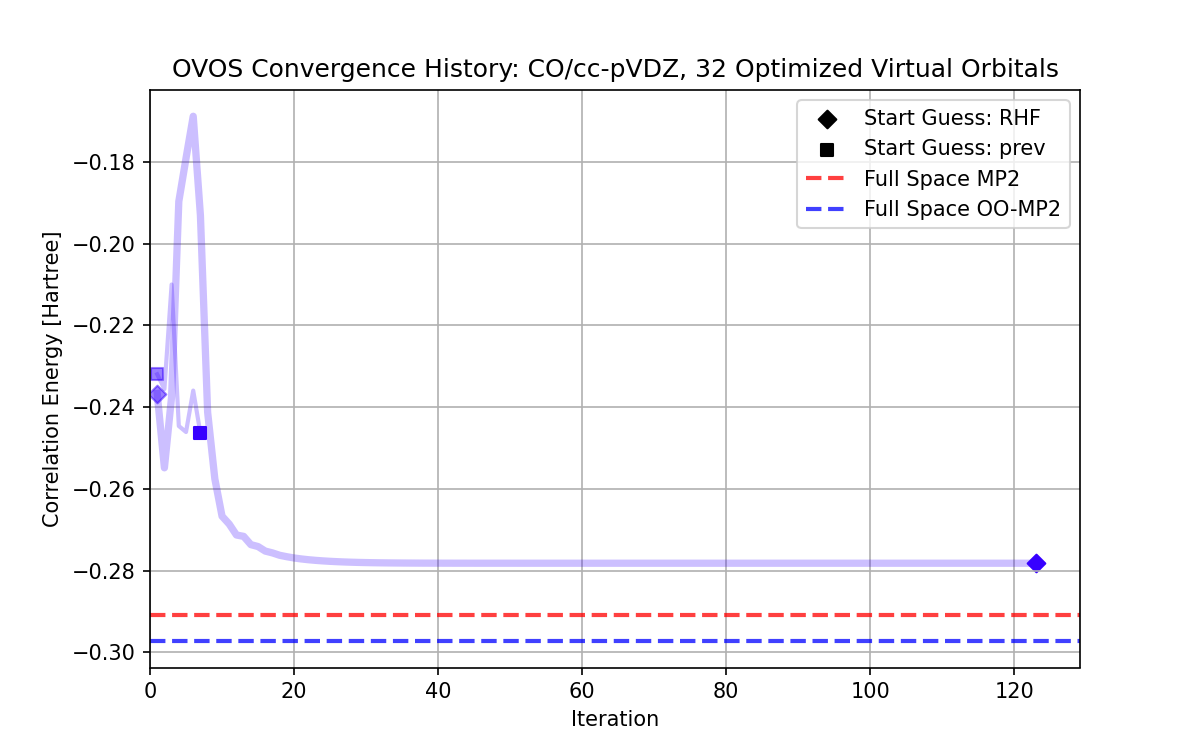
\includegraphics[width=1.0\textwidth]{figures/OVOS_PLOTS/CO/cc-pVDZ/convergence_histories/ovos_convergence_history_CO_cc-pVDZ_32_virt_orbs.png}
%     \caption{Convergence behavior of the MP2 correlation energy for ... in the ... basis with $N'_{\rm act.unocc} = ...$ active virtual spin-orbitals.}
%     \label{fig:HF_6-31G_convergence}
% \end{figure}

\subsection{Basis Set Dependence}
% ---------------------------------------------------------------
% [SECTION INTRO – 6.5]
%   "The dimension of the virtual orbital space grows rapidly with
%    basis set size, affecting both the absolute correlation energy
%    and the fraction captured by a fixed $N'$. This section
%    investigates how the $\eta$-vs-$N'$ curve changes across basis sets."
%
% [WHAT TO COVER]
%   - Compare 6-31G, cc-pVDZ, cc-pVTZ for one or two molecules (e.g. CH\textsubscript{2}, N\textsubscript{2}).
%   - Key question: does a larger basis set require proportionally more
%     active virtuals to achieve the same $\eta$?
%   - Discuss physical interpretation: larger basis has more diffuse
%     functions; their contribution to dynamical correlation.
%
% [FIGURE]
%   x-axis: $N'_{\rm act.unocc}/N_{\rm act.unocc}$ | y-axis: $\eta$
%   One curve per basis set; dashed line at $\eta=0.9$.
%   Caption: ``Basis set dependence of energy recovery for [molecule].
%   A larger basis set (more virtual orbitals) shifts the curve to the right,
%   requiring a larger fraction of active virtuals for the same $\eta$.''
%
% [LEAD-IN TO §6.6]
%   "A direct numerical comparison with the results published by
%    Adamowicz \& Bartlett is made in the following section."
% ---------------------------------------------------------------

As the OVOS algorithm optimises the orbitals to recover correlation energy, the choice of basis set influence the number of virtual orbitals and their character, which in turn affects the energy recovery. In this section, I compare the energy recovery curves for different basis sets (6--31G, cc--pVDZ) for the benchmarked molecules. We use the best results of initialisation strategies based on the results from the previous section.

\subsubsection*{CO}

Observing the correlated energy curves for CO in the 6--31G (11) and cc--pVDZ (21) basis sets, we see that the larger cc--pVDZ basis set, which has more virtual orbitals, allows for a higher fraction of correlation energy to be recovered at lower $N'_{\rm act.unocc}$. At $N'_{\rm act.unocc} = 25\%$ of the total active virtual orbitals, the cc--pVDZ basis recovers less than 6--31G basis, for which as $N'_{\rm act.unocc}$ increases, the two basis sets show similar trends. The energy recovery curves for CO in the 6--31G and cc--pVDZ basis sets are shown in Figure~\ref{fig:CO_basis_comparison}.

If instead we looked at a fixed number of active virtual orbitals, $N'_{\rm act.unocc} = 5$, their percentages of the total active virtual orbitals are different for the two basis sets, with 6--31G having a higher percentage than cc--pVDZ. We can find this point by counting 5 points along the line for each basis set in Figure~\ref{fig:CO_basis_comparison}. At this fixed number of active virtual orbitals, the 6--31G basis recovers a higher fraction of correlation energy than the cc--pVDZ basis, as the total number of virtual orbitals is smaller in 6--31G. 

\begin{figure}[H]
    \centering
    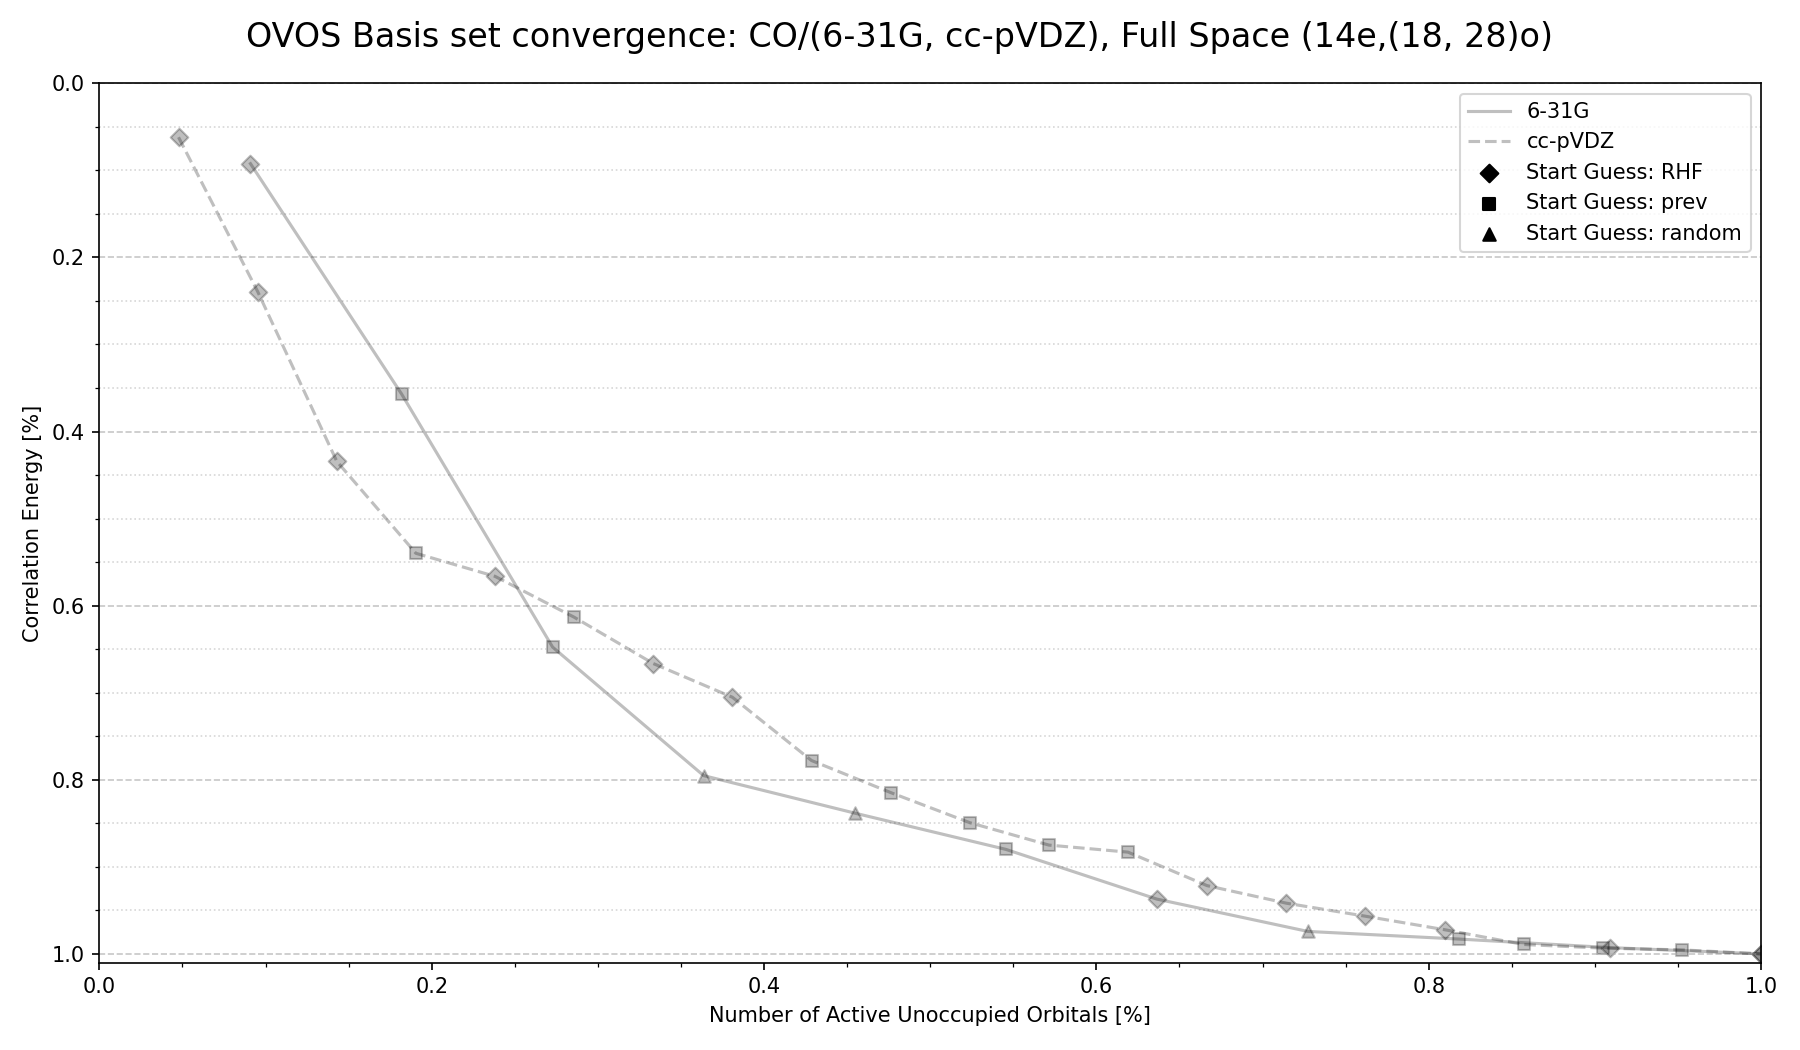
\includegraphics[width=0.9\textwidth]{figures/OVOS_PLOTS/CO/ovos_basis_set_CO_['6-31G', 'cc-pVDZ'].png}
    \caption{Basis set dependence of energy recovery for CO. The MP2 energy correlation is plotted against the active virtual orbitals for the basis sets: 6--31G (stripped) and cc--pVDZ (full) line.}
    \label{fig:CO_basis_comparison}
\end{figure}

\newpage

\subsubsection*{H2O}

The correlated energy curves for H2O in the 6--31G (8) and cc--pVDZ (19) basis sets show a stronger trend in the larger cc--pVDZ basis set, beating the smaller 6--31G basis set at most points along the curve, see Figure~\ref{fig:H2O_basis_comparison}. At $N'_{\rm act.unocc} = 25\%$ of the total active virtual orbitals, the cc--pVDZ basis recovers more correlation energy than the 6--31G basis. As $N'_{\rm act.unocc}$ increases, the two basis sets show similar trends, with the cc--pVDZ basis meeting the 6--31G basis. At a fixed number of active virtual orbitals, $N'_{\rm act.unocc} = 5$, the 6--31G basis recovers a higher correlation energy than the cc--pVDZ basis, as the total number of virtual orbitals is smaller in 6--31G.

\begin{figure}[H]
    \centering
    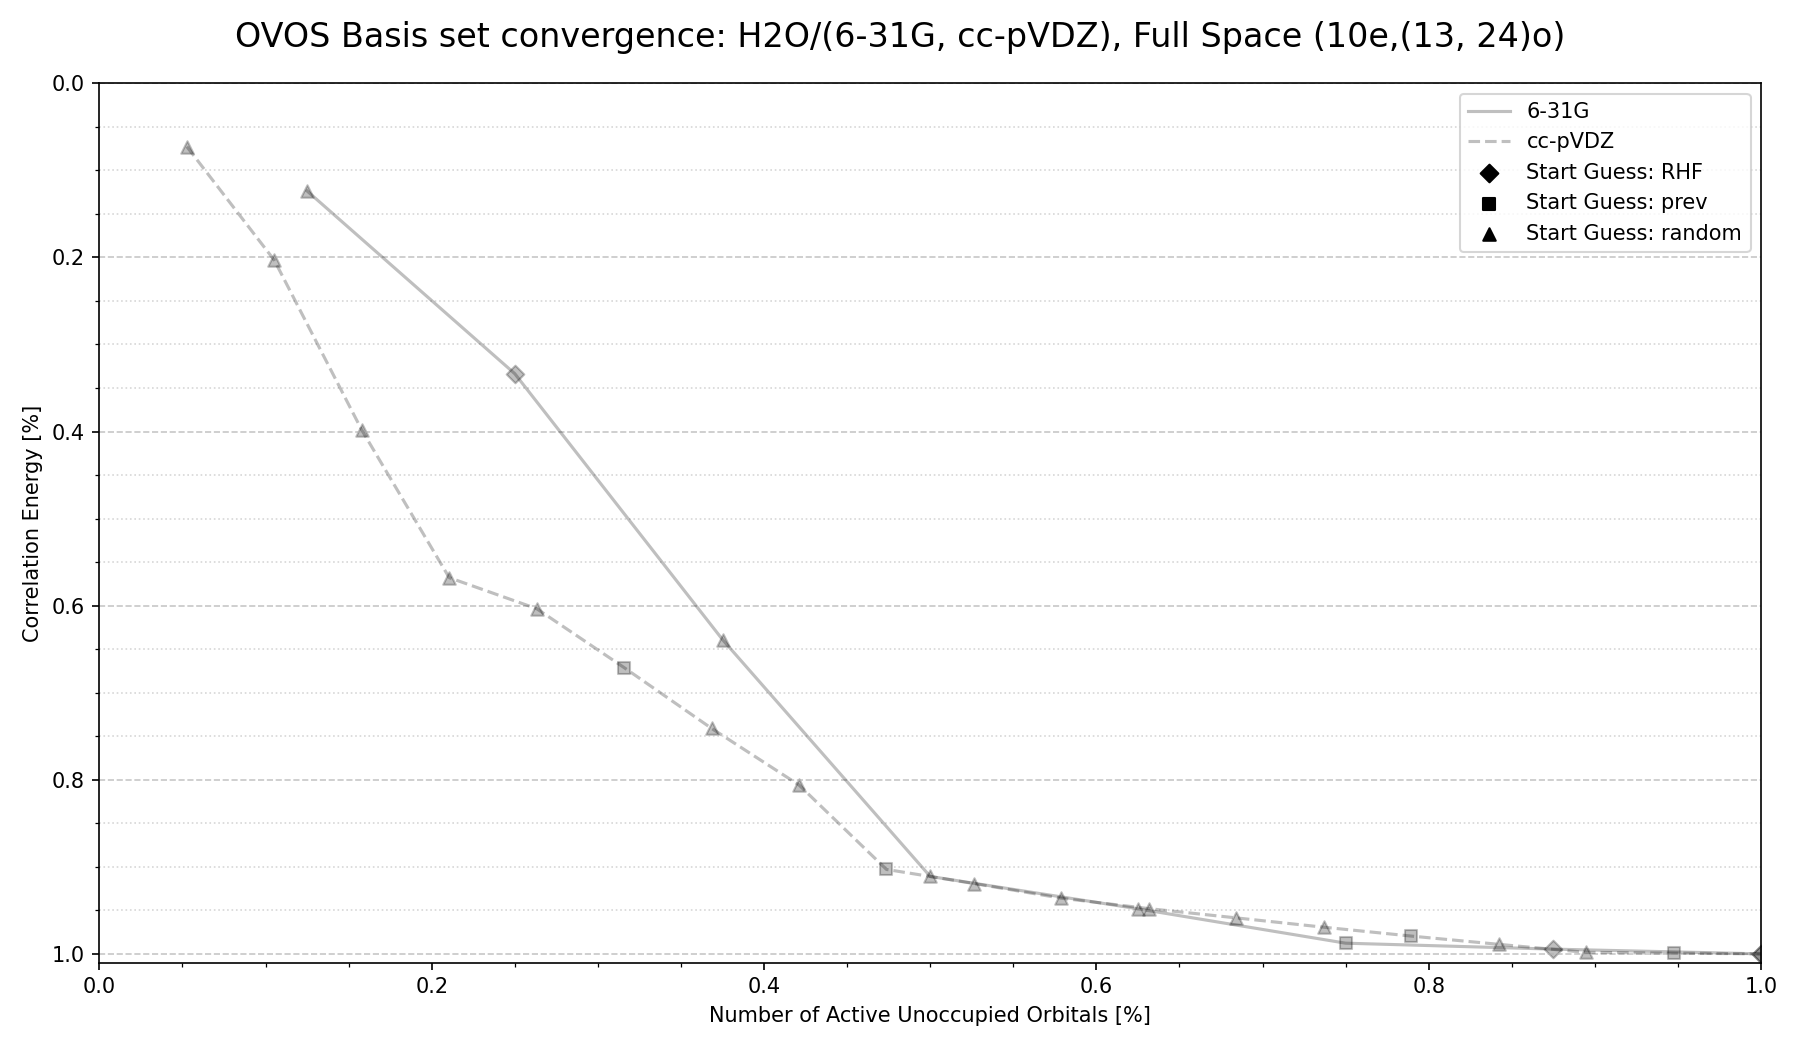
\includegraphics[width=0.9\textwidth]{figures/OVOS_PLOTS/H2O/ovos_basis_set_H2O_['6-31G', 'cc-pVDZ'].png}
    \caption{Basis set dependence of energy recovery for H2O. The MP2 energy correlation is plotted against the active virtual orbitals for the basis sets: 6--31G (stripped) and cc--pVDZ (full) line.}
    \label{fig:H2O_basis_comparison}
\end{figure}


\subsubsection*{HF}

The correlated energy curves for HF in the 6--31G (6) and cc--pVDZ (14) basis sets show a stronger trend in the larger cc--pVDZ basis set, beating the smaller 6--31G basis set at most points along the curve, see Figure~\ref{fig:HF_basis_comparison}. At $N'_{\rm act.unocc} = 25\%$ of the total active virtual orbitals, the cc--pVDZ basis recovers more correlation energy than the 6--31G basis. As $N'_{\rm act.unocc}$ increases, the two basis sets show similar trends, with the cc--pVDZ basis meeting the 6--31G basis. At a fixed number of active virtual orbitals, $N'_{\rm act.unocc} = 5$, the 6--31G basis recovers a higher correlation energy than the cc--pVDZ basis, as the total number of virtual orbitals is smaller in 6--31G.

\begin{figure}[H]
    \centering
    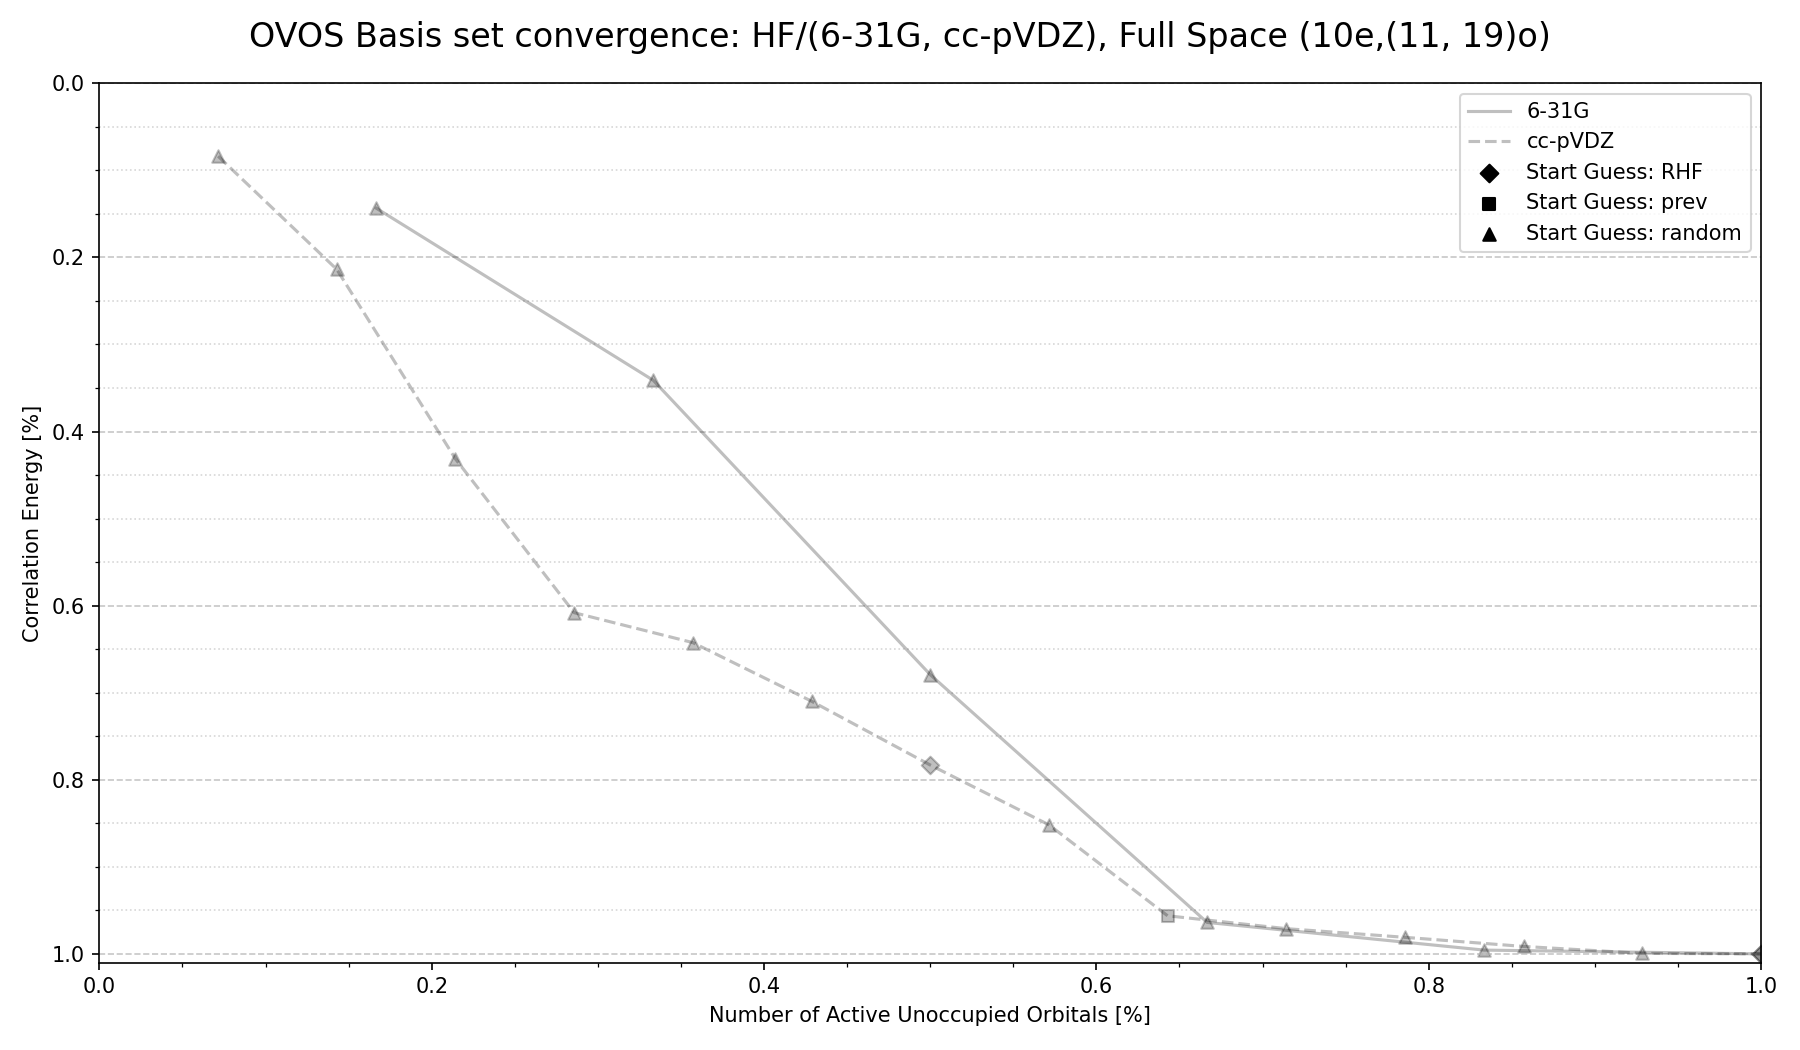
\includegraphics[width=0.9\textwidth]{figures/OVOS_PLOTS/HF/ovos_basis_set_HF_['6-31G', 'cc-pVDZ'].png}
    \caption{Basis set dependence of energy recovery for HF. The MP2 energy correlation is plotted against the active virtual orbitals for the basis sets: 6--31G (stripped) and cc--pVDZ (full) line.}
    \label{fig:HF_basis_comparison}
\end{figure}

\subsubsection*{NH3}

% 6-31G (10) and cc--pVDZ (24) 

The correlated energy curves for NH3 in the 6--31G (10) and cc--pVDZ (24) basis sets show a stronger trend in the larger cc--pVDZ basis set, beating the smaller 6--31G basis set at most points along the curve, see Figure~\ref{fig:NH3_basis_comparison}. At $N'_{\rm act.unocc} = 25\%$ of the total active virtual orbitals, the cc--pVDZ basis recovers more correlation energy than the 6--31G basis. As $N'_{\rm act.unocc}$ increases, the two basis sets show similar trends, with the cc--pVDZ basis meeting the 6--31G basis. At a fixed number of active virtual orbitals, $N'_{\rm act.unocc} = 5$, the 6--31G basis recovers a higher correlation energy than the cc--pVDZ basis, as the total number of virtual orbitals is smaller in 6--31G.

\begin{figure}[h]
    \centering
    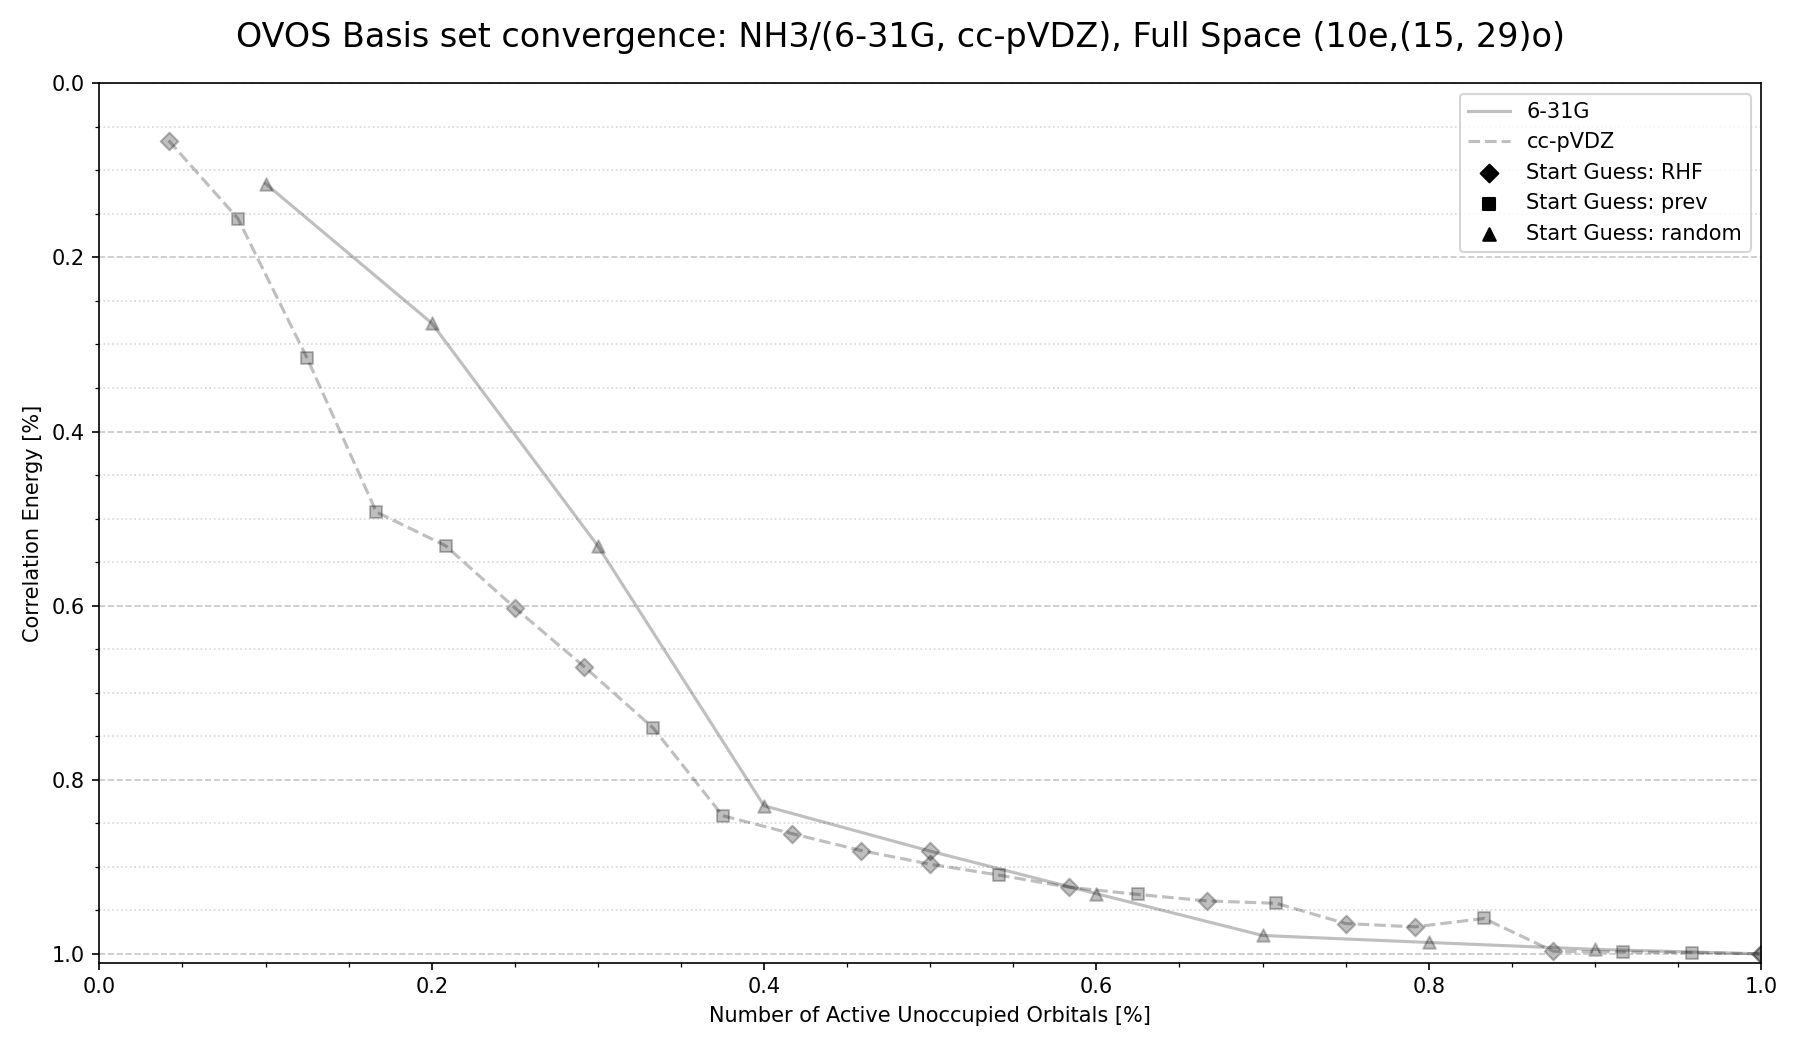
\includegraphics[width=0.9\textwidth]{figures/OVOS_PLOTS/NH3/ovos_basis_set_NH3_['6-31G', 'cc-pVDZ'].png}
    \caption{Basis set dependence of energy recovery for NH3. The MP2 energy correlation is plotted against the active virtual orbitals for the basis sets: 6--31G (stripped) and cc--pVDZ (full) line.}
    \label{fig:NH3_basis_comparison}
\end{figure}

\subsubsection*{Li2}

% 6-31G (15) and cc--pVDZ (25) 

The correlated energy curves for Li2 in the 6--31G (15) and cc--pVDZ (25) basis sets show a similar trend, with the cc--pVDZ basis set generally recovering more correlation energy than the 6--31G basis set. This is consistent with the observations for previous molecules, where larger basis sets tend to perform better in terms of energy recovery, especially at lower $N'_{\rm act.unocc}$. At $N'_{\rm act.unocc} = 25\%$ of the total active virtual orbitals, the cc--pVDZ basis recovers more correlation energy than the 6--31G basis. As $N'_{\rm act.unocc}$ increases, the two basis sets show similar trends, with the cc--pVDZ basis meeting the 6--31G basis. Where when they get to the bad points of cc--pVDZ, the 6--31G basis performs better. At a fixed number of active virtual orbitals, $N'_{\rm act.unocc} = 5$, the 6--31G basis recovers a higher correlation energy than the cc--pVDZ basis, as the total number of virtual orbitals is smaller in 6--31G.


\begin{figure}[H]
    \centering
    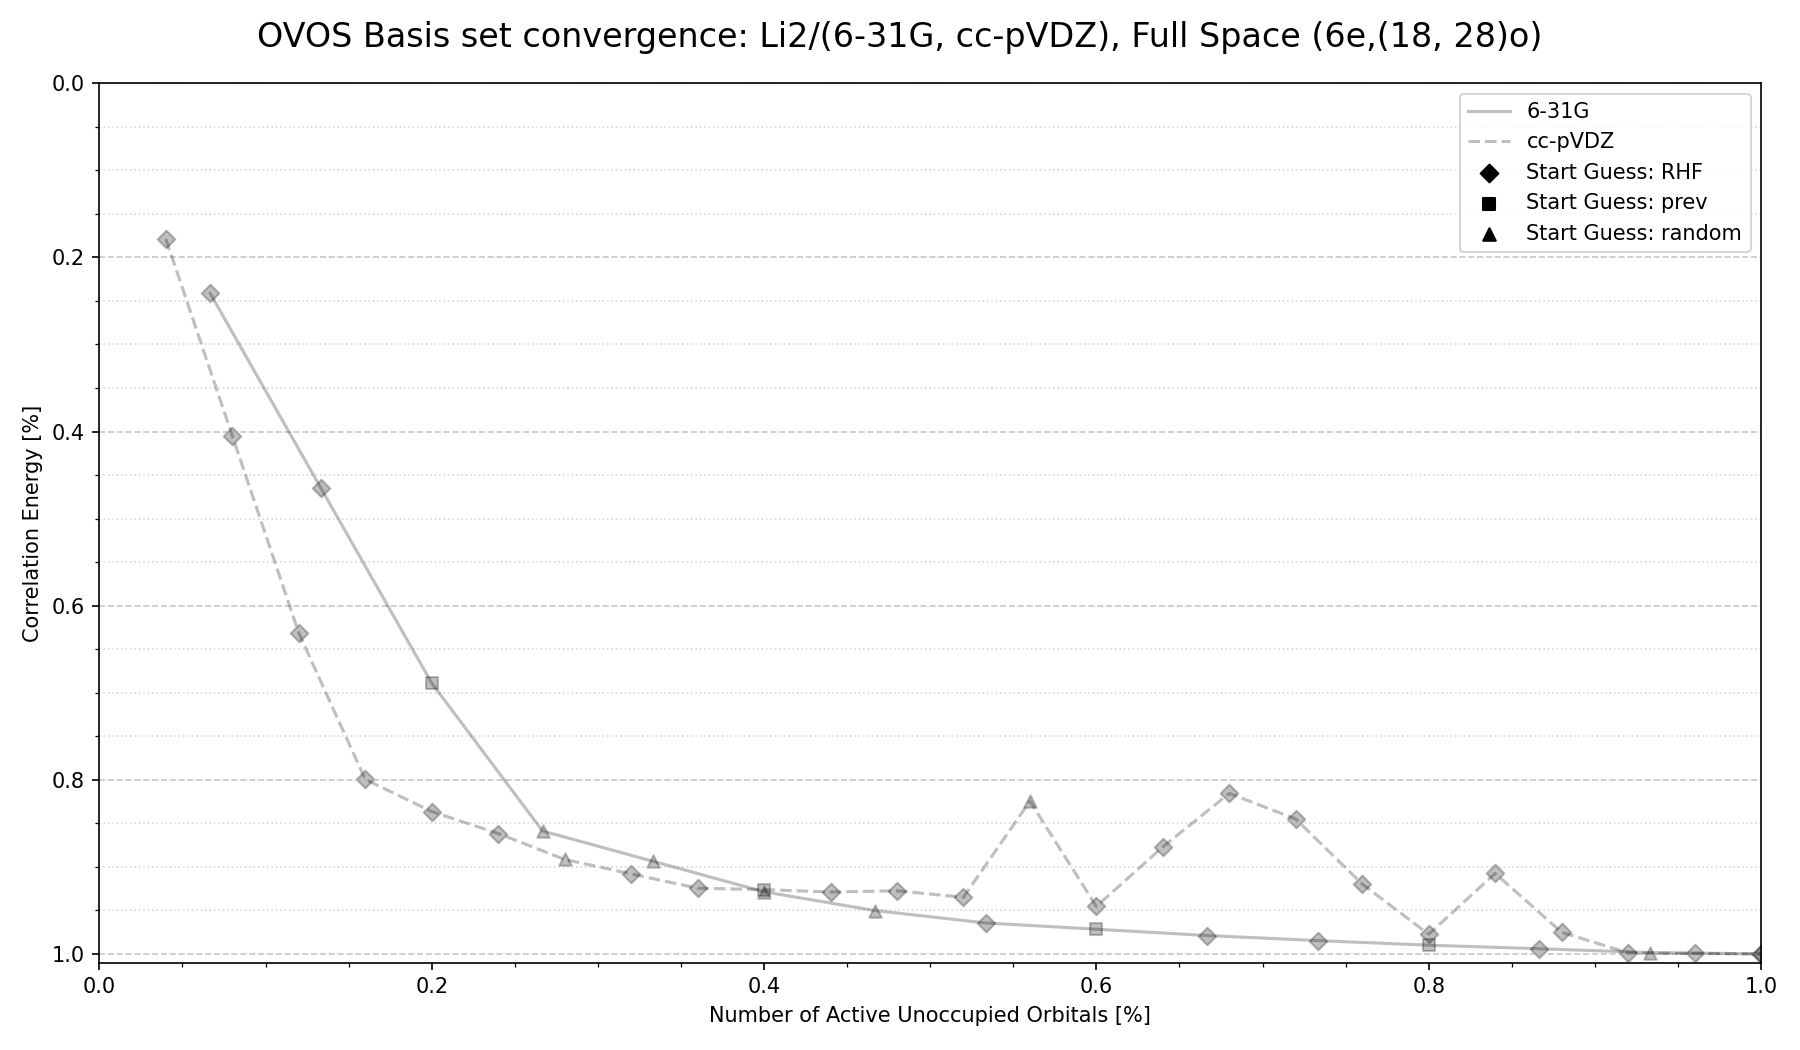
\includegraphics[width=0.9\textwidth]{figures/OVOS_PLOTS/Li2/ovos_basis_set_Li2_['6-31G', 'cc-pVDZ'].png}
    \caption{Basis set dependence of energy recovery for Li2. The MP2 energy correlation is plotted against the active virtual orbitals for the basis sets: 6--31G (stripped) and cc--pVDZ (full) line.}
    \label{fig:Li2_basis_comparison}
\end{figure}



% For the bigger basis set cc--pVDZ, at the number of virtual space of the smaller 6--31G set for active virtual space, we can recover a better correlation energy than at full space in 6--31G...

% If instead we fix the absolute number of active unoccupied orbitals, we can recover a higher fraction of correlation energy in a smaller basis set, as the total number of virtual orbitals is smaller...

% Instead we flip it and make a sat procentage of the active unoccupied orbitals, we can recover a better correlation energy in a bigger basis set, as the total number of virtual orbitals is smaller, as seen in ... 

% These results indicate that the choice of basis set has a significant impact on the energy recovery behaviour of the OVOS algorithm, a larger basis set means more mixing options translating to a better correlation energy...


\subsubsection{Comparison with Adamowicz and Bartlett (1987)}
% ---------------------------------------------------------------
% [SECTION INTRO – 6.6]
%   "The benchmark test case of Adamowicz \& Bartlett \cite{Adamowicz1987}
%    is the CH\textsubscript{2} molecule (triplet ground state). This section
%    compares the OVOS energy recovery curves obtained in this work with
%    those reported in Table I of the original paper."
%
% [WHAT TO COVER]
%   - Direct comparison of $E_{\rm corr}(N')$ for CH\textsubscript{2}.
%   - Discuss differences: UHF vs.~RHF reference, basis set version, geometry.
%   - Consider showing a small table with side-by-side values.
%   - If agreement is within expected accuracy: confirms correctness.
%   - If differences: explain and quantify their source.
%
% [TABLE]
%   Columns: $N'_{\rm act.unocc}$ | $E_{\rm corr}^{\rm A\&B}$ |
%            $E_{\rm corr}^{\rm this work}$ | Difference
%   Caption: ``Comparison of OVOS correlation energies for
%   CH\textsubscript{2} with values from Adamowicz \& Bartlett
%   \cite{Adamowicz1987}. Differences may arise from basis set
%   and reference wavefunction choices.''
%
% [LEAD-IN TO §6.7]
%   "The computational efficiency of the OVOS algorithm, and how
%    it scales with system and basis set size, is assessed in
%    the following section."
% ---------------------------------------------------------------

Adamowicz \& Bartlett's 1987 paper presents OVOS results for the CH\textsubscript{2} ($^1A_1$) molecule in a (9s7p2d If,5s2p) contracted Gaussian basis set in their Table I, here they note that it has the size of $70$ active virtual orbitals \cite{Adamowicz1987}. I include their results here to show the potential of OVOS at bigger basis sets, and to compare with the results obtained in this work. However, it is important to note that there are differences in the computational details between their work and this one, such as their handling of convergence (which does not seem to be detailed, e.g. ill-conditioned Hessian, iteration count, ...), and the geometry of the molecule. These differences can lead to variations in the correlation energy values, making a direct comparison challenging.

\begin{table}[h]
    \centering
    \begin{tabular}{ccccc}
        \hline
        Molecule / N'          & 100\%     & \~50\%     & \~30\%     & \~10\% \\
        \hline
        $CH_2$$^\dagger$ (70)  & 99\%      & \~96\%     & \~88\%     & \~50\% \\
        $Li_2$           (25)  & 100\%     & \~92\%     & \~90\%     & \~50\% \\
        $NH_3$           (24)  & 100\%     & \~90\%     & \~66\%     & \~18\% \\
        $CO$             (21)  & 100\%     & \~86\%     & \~70\%     & \~22\% \\
        $H_2O$           (19)  & 100\%     & \~90\%     & \~65\%     & \~15\% \\
        $HF$             (14)  & 100\%     & \~89\%     & \~61\%     & \~16\% \\
        \hline
    \end{tabular}
    \caption{Comparison of my implementation of OVOS for other molecules in cc-pvCVZ basis set against the values from Adamowicz \& Bartlett \cite{Adamowicz1987} (noted by a $\dagger$). The energies are in percentages of the full space correlation energy for each molecule, of which in parentheses their active virtual orbital counts are given.}
    \label{tab:comparison_AB}
\end{table}

Looking past not being able to replicate the exact setup of Adamowicz \& Bartlett, the basis sets behaviour shows some similarities with their findings. It is agreeable that around 90\% of the correlation energy can be recovered with around 50\% of the active virtual orbitals. It is less agreeable for the 30\% and 10\% of the active virtual orbitals, where we see only $Li_2$ finds similar findings, despite its regions of bad convergence, see \ref{subsec:results_ovos_mp2}. The other molecules show a much lower percentage of correlation energy recovery at these lower active virtual orbital counts, which is likely due to molecular and basis set differences. Bigger basis sets might be necessary for these molecules. The comparison of the energy recovery percentages for the different molecules in this work against the values from Adamowicz \& Bartlett \cite{Adamowicz1987} are shown in Table~\ref{tab:comparison_AB}.




\section{VQE}
\label{sec:results_veq}

This section presents the non orbital optimised VQE results for the test molecules, using the OVOS-optimised orbitals as the reference state. The goal is to quantify the practical benefit of OVOS MOs for quantum computing by computing potential energy surface, the reference-state overlap, and comment their relation to Brueckner orbitals. The VQE results are compared to those obtained using the UHF orbitals and UMP2 natural orbitals as reference states, to assess the improvement in energy convergence and resource savings.

\subsection{VQE potential energy surfaces plot}
\label{sec:results_vqe}
% ---------------------------------------------------------------
% OVOS Orbitals as a VQE Reference State
% ---------------------------------------------------------------
% Goal: Quantify the practical benefit of OVOS MOs for quantum
%       computing by computing the reference-state overlap, 
%       computing energy VQE optimization ... 
%       and estimating qubit/circuit savings.
%
% Suggested analysis:
%   (a) Reference-state overlap
%       - For small molecules (H₂, LiH, H₂O in minimal/small basis),
%         compute the FCI ground state using PySCF fci.FCI().
%       - Compute the overlap F = |⟨Φ_ref|Ψ_FCI⟩|² for:
%           * |Φ_HF⟩ (standard HF reference)
%           * |Φ_OVOS⟩ (OVOS-optimised reference, varying N'_virt)
%       - Plot F_OVOS vs N'_virt/N_virt^max and compare to F_HF.
%       - Table: molecule | basis | N'_virt | F_HF | F_OVOS | ΔF
%
%   (b) VQE wavefunction optimizaton
%       - does the energy landscape become easier 
%       to navigate with OVOS orbitals?
%       - In less iterations? 
%       - With less energy fluctuations?
%       - Better energy convergence?
%
%   (c) Resource estimate
%       - Qubit count: Q = 2(N_occ + N'_virt) for JW encoding.
%       - UCCSD parameter count: N_occ * N'_virt (singles) +
%         N_occ^2 * N'_virt^2 / 4 (doubles).
%       - Tabulate Q and n_params for HF vs OVOS at η = 90% for
%         each test molecule.
%
% Notes:
%   - This section is primarily theoretical/numerical estimation;
%     actual VQE circuit runs are outside the scope of this thesis
%     (discussed in Outlook §8.3).
%   - Cite \cite{Peruzzo2014, Cao2019, deGracia2024, Seeley2012}
%     for VQE and qubit encoding background.
% ---------------------------------------------------------------

Below I present the potential energy surfaces for H2O, HF, and Li2 for the VQE calculations using the OVOS-optimised orbitals as reference states. Here, the VQE calculations are performed without orbital optimization, as detailed in Section~\ref{sec:methods_vqe}, and the results are compared to those obtained using the UHF orbitals and UMP2 natural orbitals as reference states. When it comes to potential energy surfaces, a common way to visualize the performance of different reference states is to plot the energy as a function of a reaction coordinate, such as bond length or angle, for each reference state. This allows us to see how well the VQE calculations converge to the true ground state energy across different geometries. The plot will highlight if the orbitals dissociates correctly, and if the energy convergence is smooth or if there are any irregularities. The goal is to assess the improvement in energy convergence when using OVOS-optimised orbitals for VQE calculations.

% "Comment on VQE results for ... in the ... basis, with the OVOS orbitals as reference state, compared to the UHF orbitals, and UMP2 natural orbitals as reference state. Comment on iteration and energy in VQE calculations using orbital optimization or not. Comment on random initialization of thetas vs previous geometry final values... Comment on the qubit savings and parameter savings... "

\subsubsection*{H2O}

For H2O, in 6-31G basis set, the VQE calculations using the OVOS-optimised orbitals as reference states show a consistent small improvement over the UHF orbitals, with a lower energy convergence. Both the OVOS-optimised orbitals and UHF orbitals show a smooth potential energy surface, along with correct dissociation behavior, with the OVOS-optimised orbitals showing a slightly better convergence to the true ground state energy across different geometries. The UMP2 natural orbitals, show a even lower energy convergence than the UHF orbitals and OVOS-optimised orbitals, which is expected given that they are typically considered to be better reference states for correlated calculations. The OVOS-optimised orbitals seems to catch up to the UMP2 natural orbitals in terms of energy convergence after dissociation. Observing the plots conmpared to the reference UHF curve, the VQE calculations all show improved convergence across the potential energy surface. The potential energy surfaces for H2O using the OVOS-optimised orbitals, UHF orbitals, and UMP2 natural orbitals as reference states are shown in Figure~\ref{fig:H2O_VQE_false.png}. 

\begin{figure}[H]
    \centering
    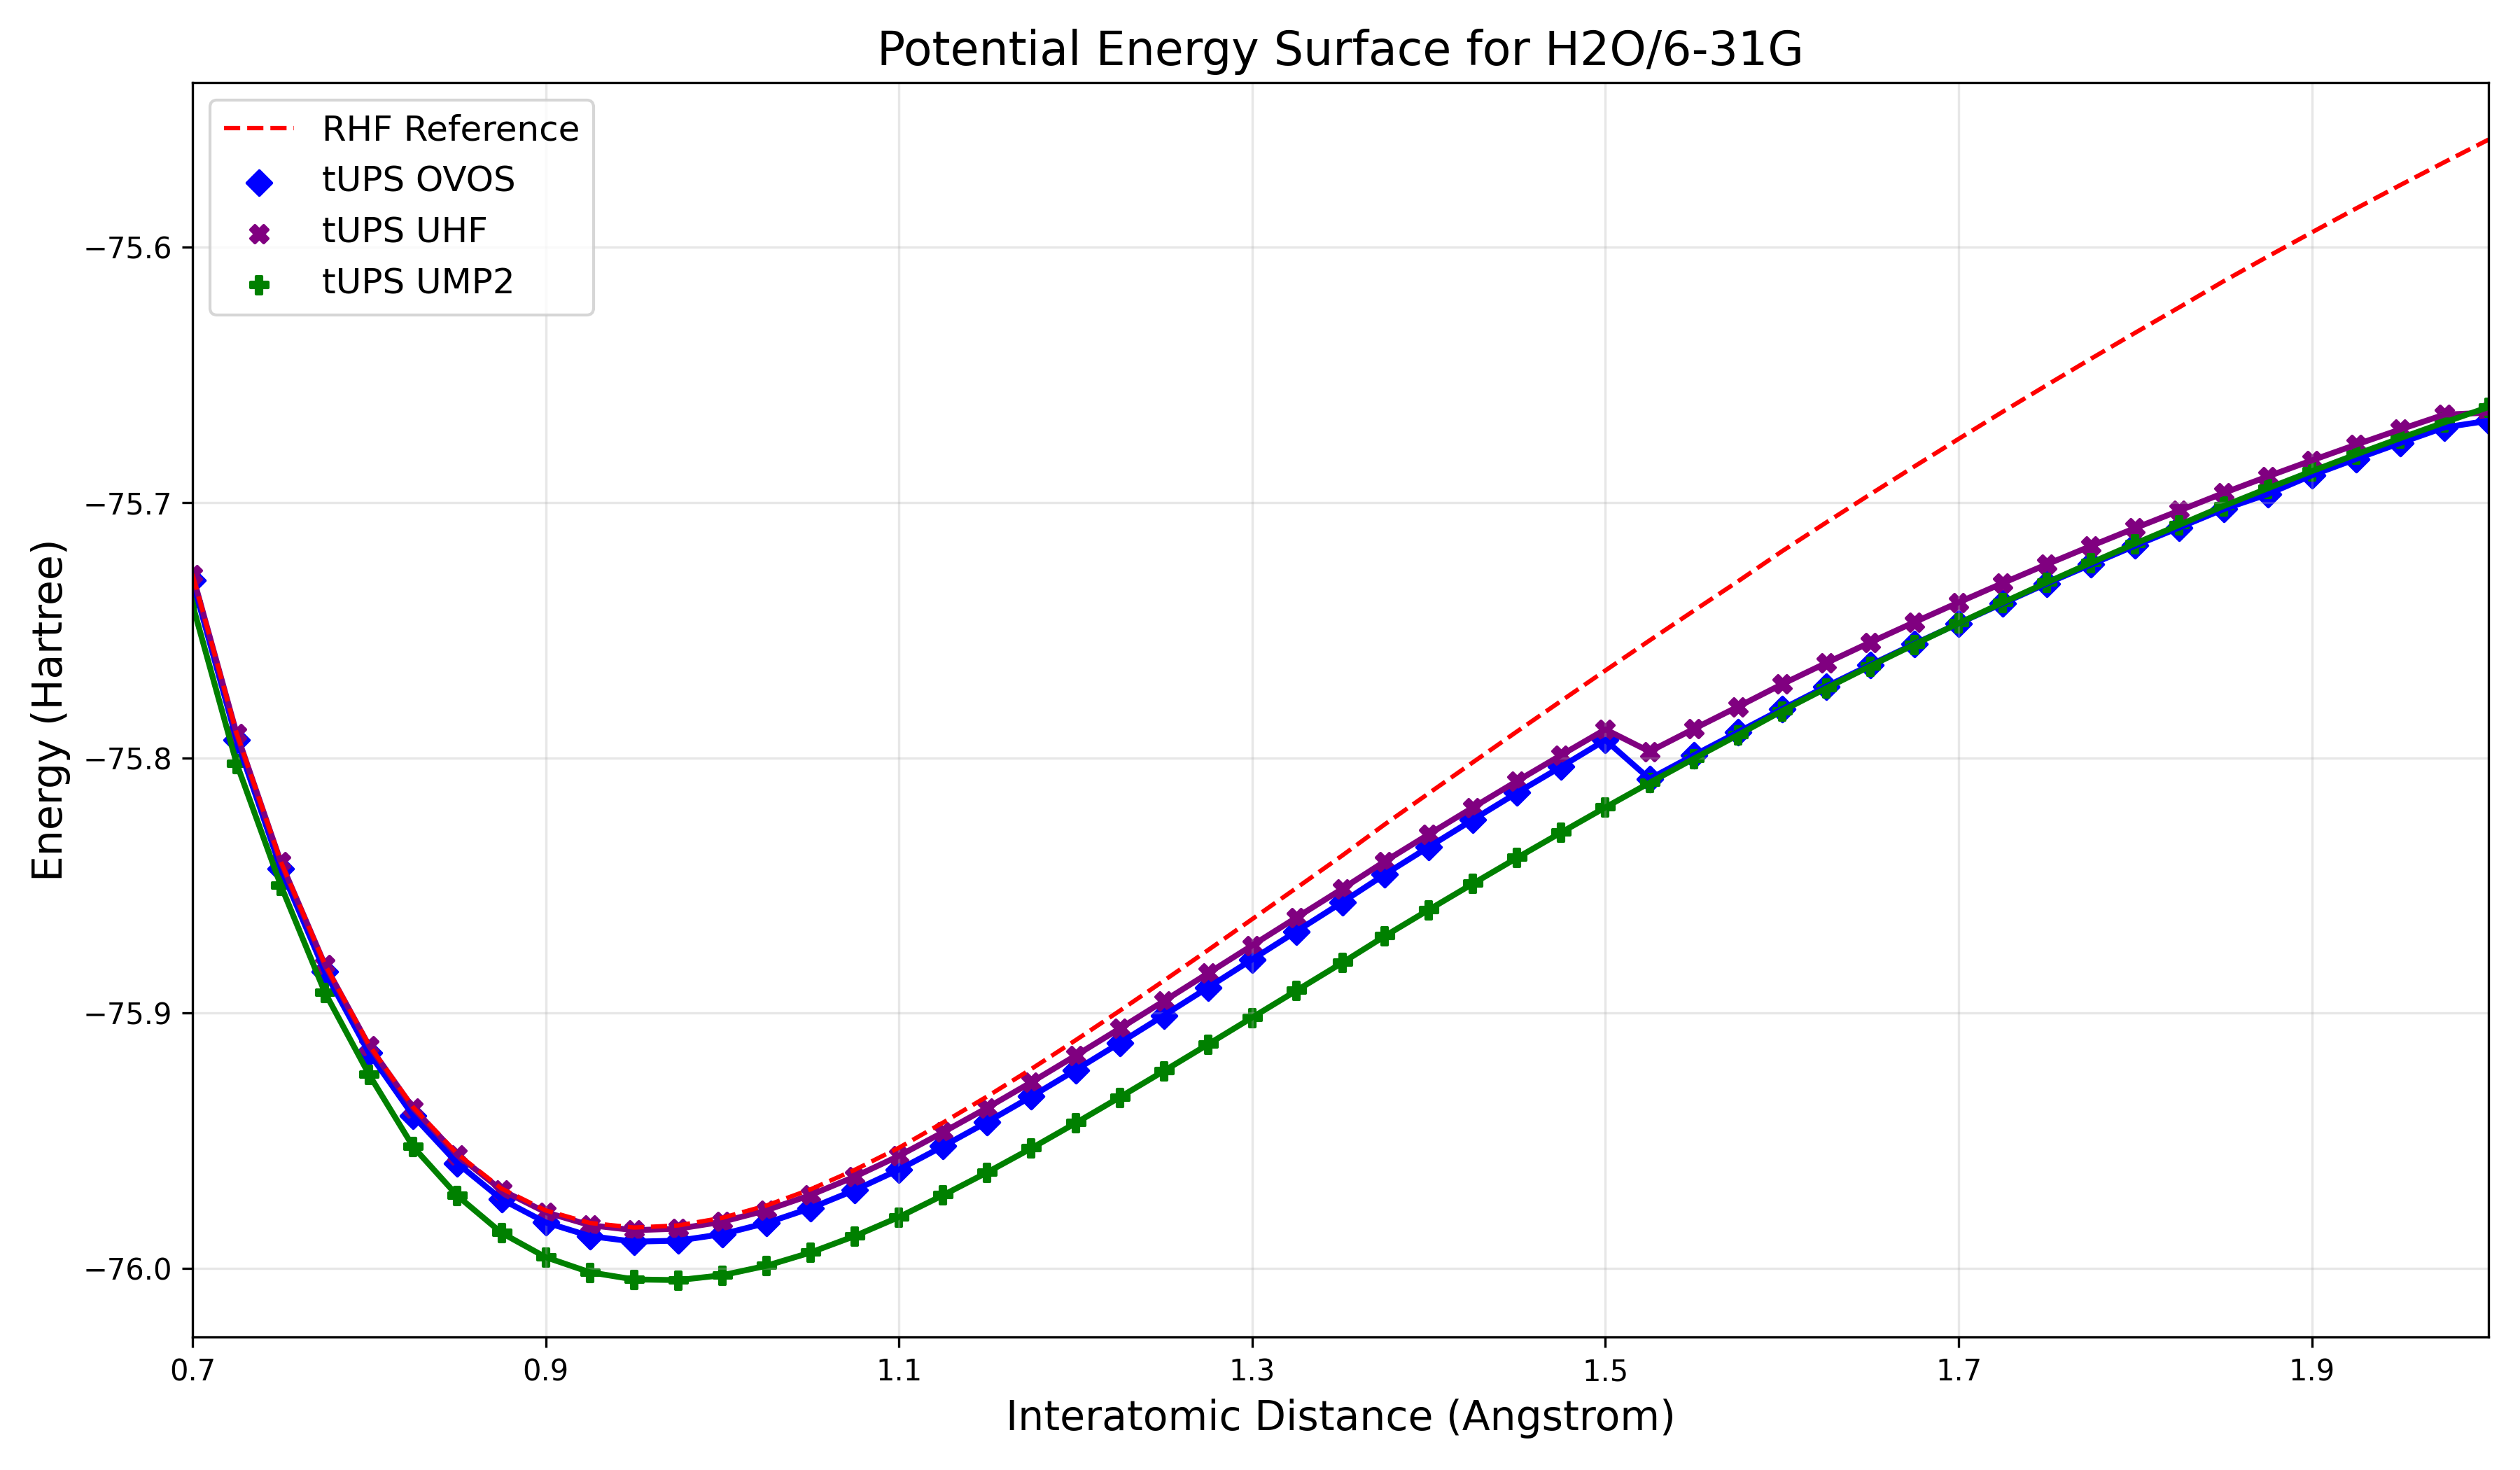
\includegraphics[width=0.9\textwidth]{figures/VQE_PLOTS/H2O/VQE_H2O_6-31G_best_of_zoom_oo_False.png}
    \caption{Potential energy surfaces for H2O in 6-31G basis set, using the OVOS-optimised orbitals (blue), UHF orbitals (purple), and UMP2 natural orbitals (green) as reference states in VQE calculations. The active space is the same for all calculations with 10 electrons and 6 virtual orbitals (75\% of the full virtual space). The dashed lines represent the reference energies from PySCF. The plot shows the energy convergence across different geometries.}
    \label{fig:H2O_VQE_false.png}
\end{figure}

\subsubsection*{HF}

For HF, in 6-31G basis set, the VQE calculations using the OVOS-optimised orbitals as reference states show a consistent improvement over the UHF orbitals, with a lower energy convergence, up untill it shows dissociation behavior, where the UHF orbitals show a better convergence. Both the OVOS-optimised orbitals and UHF orbitals show a smooth potential energy surface, along with dissociation behavior occuring a interatomic distance later at $1.32$ Å. The UMP2 natural orbitals, are catched up by the UHF orbitals after dissociation, and show a better convergence than the OVOS-optimised orbitals across the potential energy surface. Observing the plots conmpared to the reference UHF curves, the VQE calculations, except for the UHF orbitals before dissociation, show improved convergence across the potential energy surface. The potential energy surfaces for HF using the OVOS-optimised orbitals, UHF orbitals, and UMP2 natural orbitals as reference states are shown in Figure~\ref{fig:HF_VQE_false.png}.

\begin{figure}[H]
    \centering
    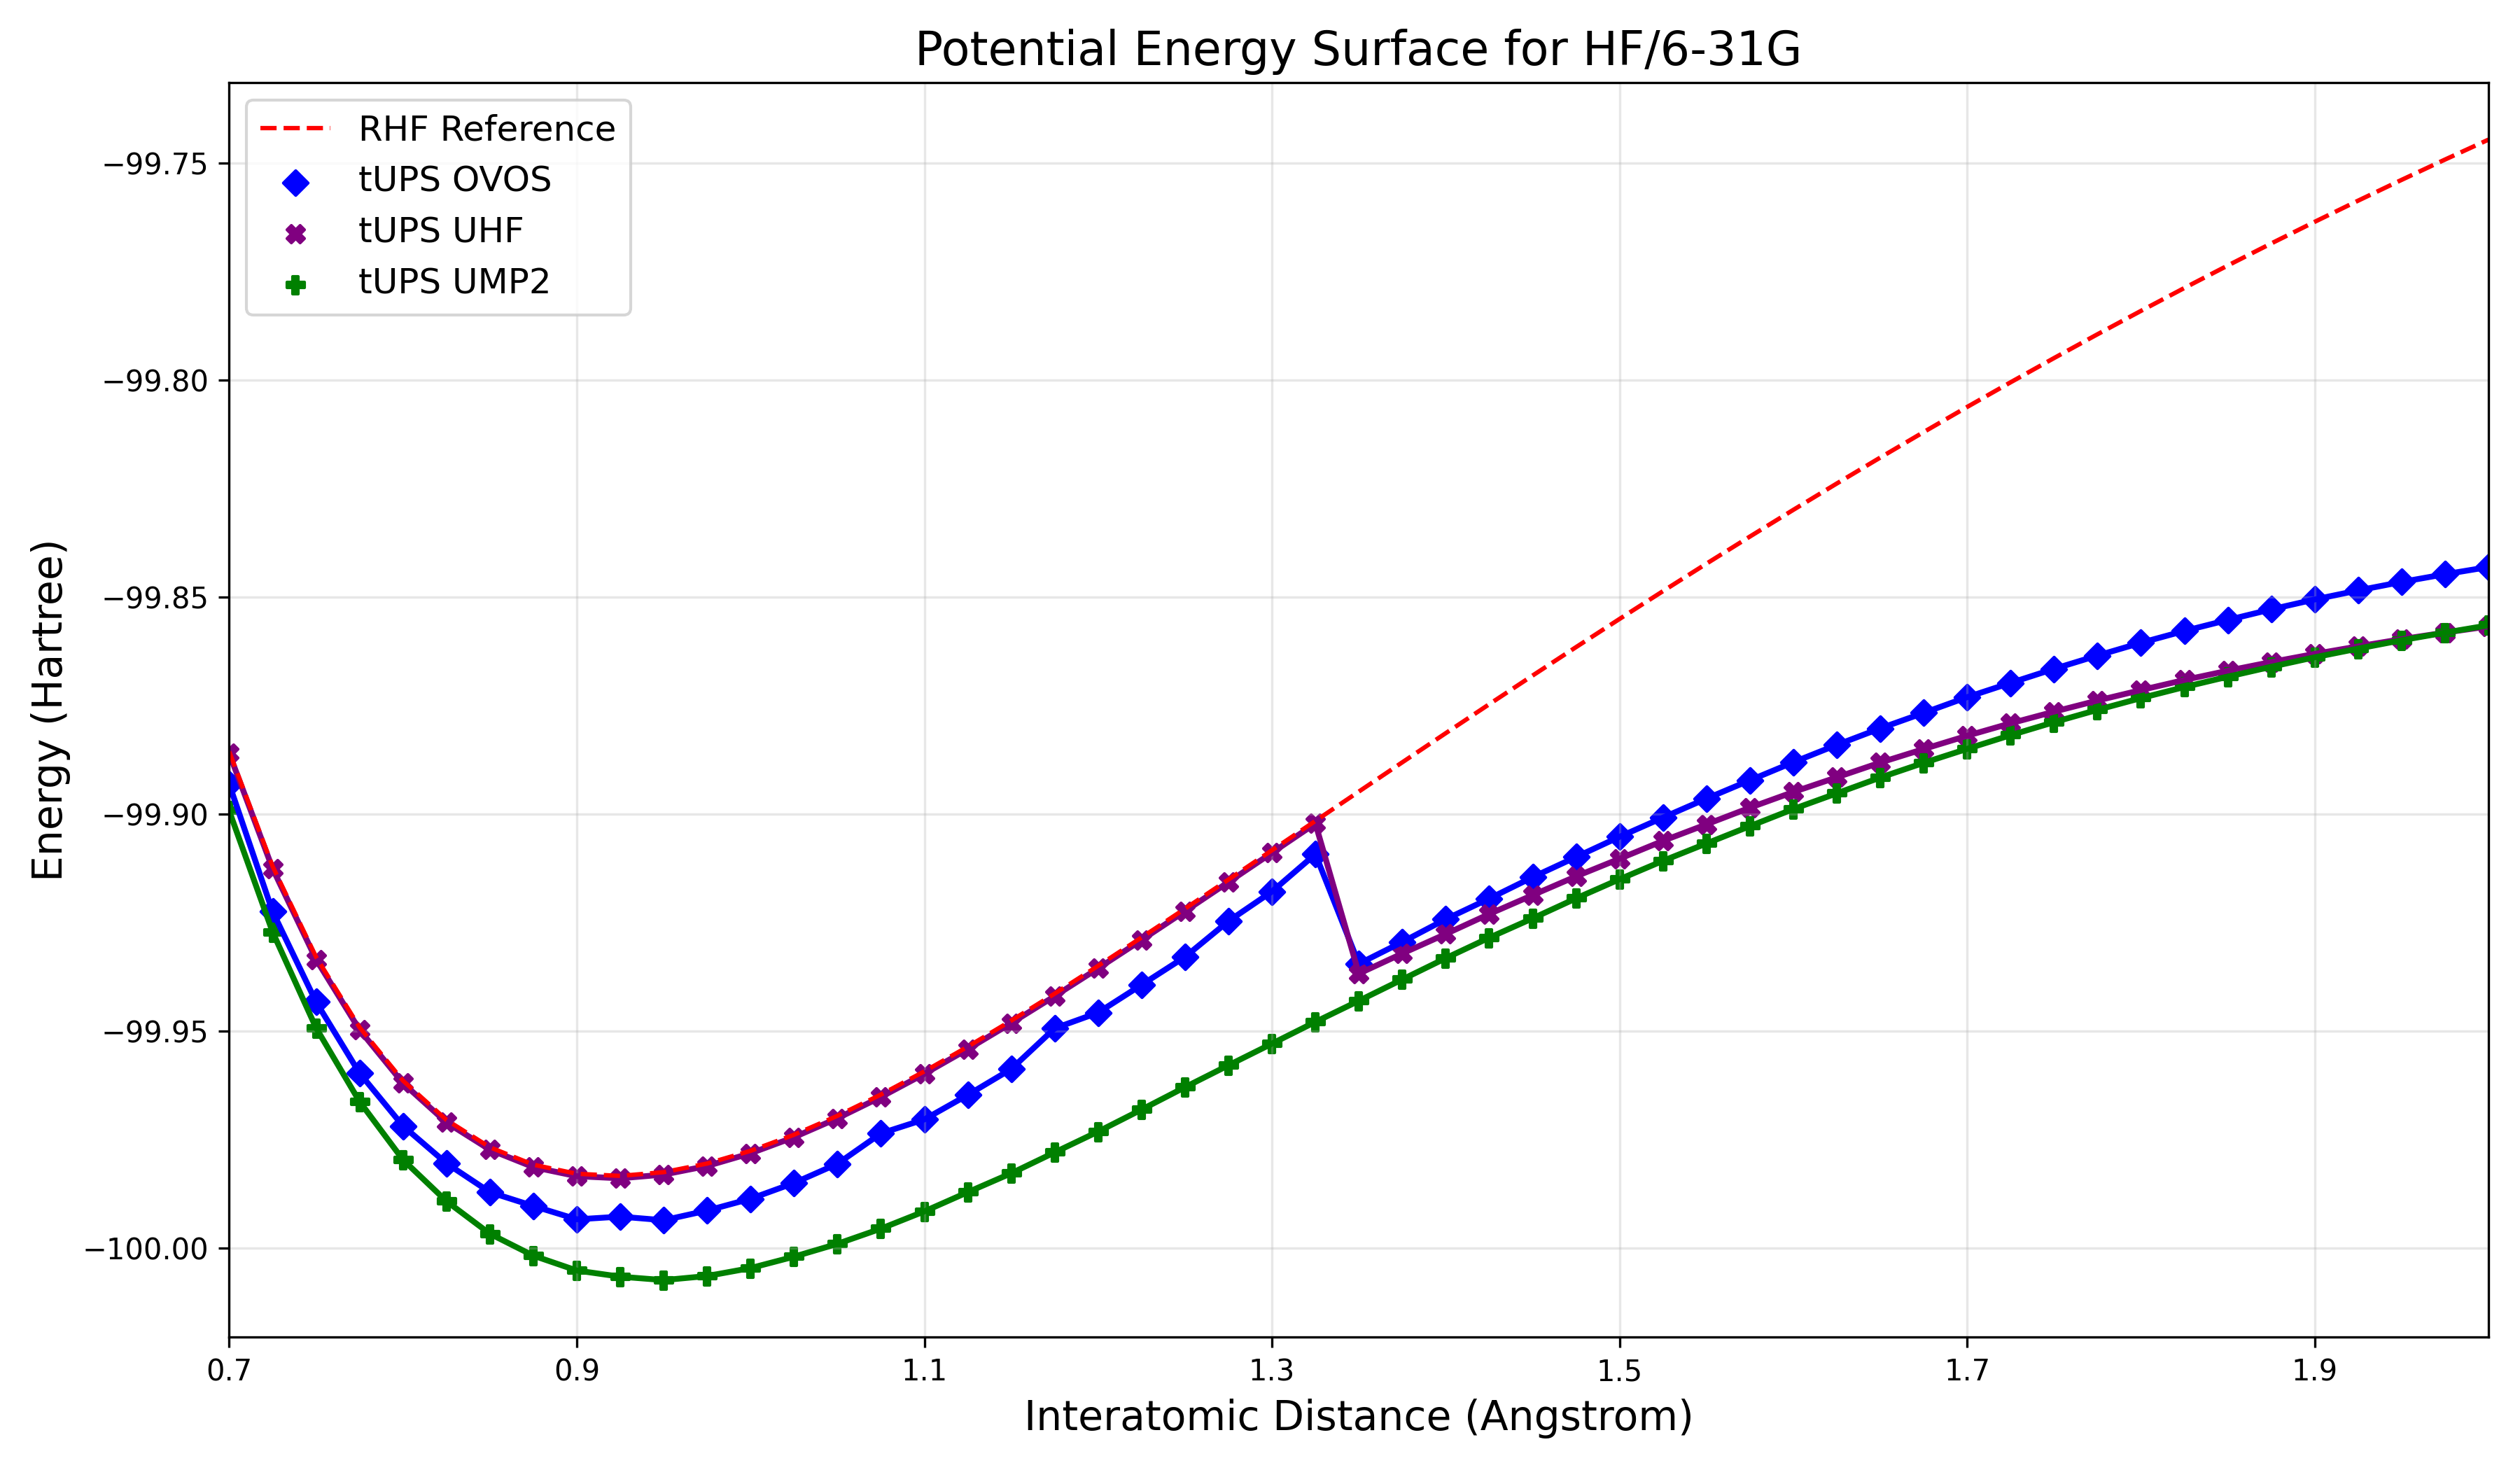
\includegraphics[width=0.9\textwidth]{figures/VQE_PLOTS/HF/VQE_HF_6-31G_best_of_zoom_oo_False.png}
    \caption{Potential energy surfaces for HF in 6-31G basis set, using the OVOS-optimised orbitals (blue), UHF orbitals (purple), and UMP2 natural orbitals (green) as reference states in VQE calculations. The active space is the same for all calculations with 10 electrons and 5 virtual orbitals (75\% of the full virtual space rounded up). The dashed lines represent the reference energies from PySCF.  The plot shows the energy convergence across different geometries.}
    \label{fig:HF_VQE_false.png}
\end{figure}

\subsubsection*{Li2}

For Li2, in 6-31G basis set, the VQE calculations using the OVOS-optimised orbitals as reference states show a consistent improvement over the UHF orbitals, with a lower energy convergence. Both the OVOS-optimised orbitals and UHF orbitals does not show a smooth potential energy surface, still the UMP2 natural orbitals show a smooth potential energy surface. The UMP2 natural orbitals, show a better energy convergence than the UHF orbitals and OVOS-optimised orbitals, which is expected given that they are typically considered to be better reference states for correlated calculations. The OVOS-optimised orbitals never catches up to the UMP2 natural orbitals in terms of energy convergence after dissociation. Observing the plots conmpared to the reference UHF curve, all VQE calculations show improved convergence across the potential energy surface. The potential energy surfaces for Li2 using the OVOS-optimised orbitals, UHF orbitals, and UMP2 natural orbitals as reference states are shown in Figure~\ref{fig:Li2_VQE_false.png}.

\begin{figure}[H]
    \centering
    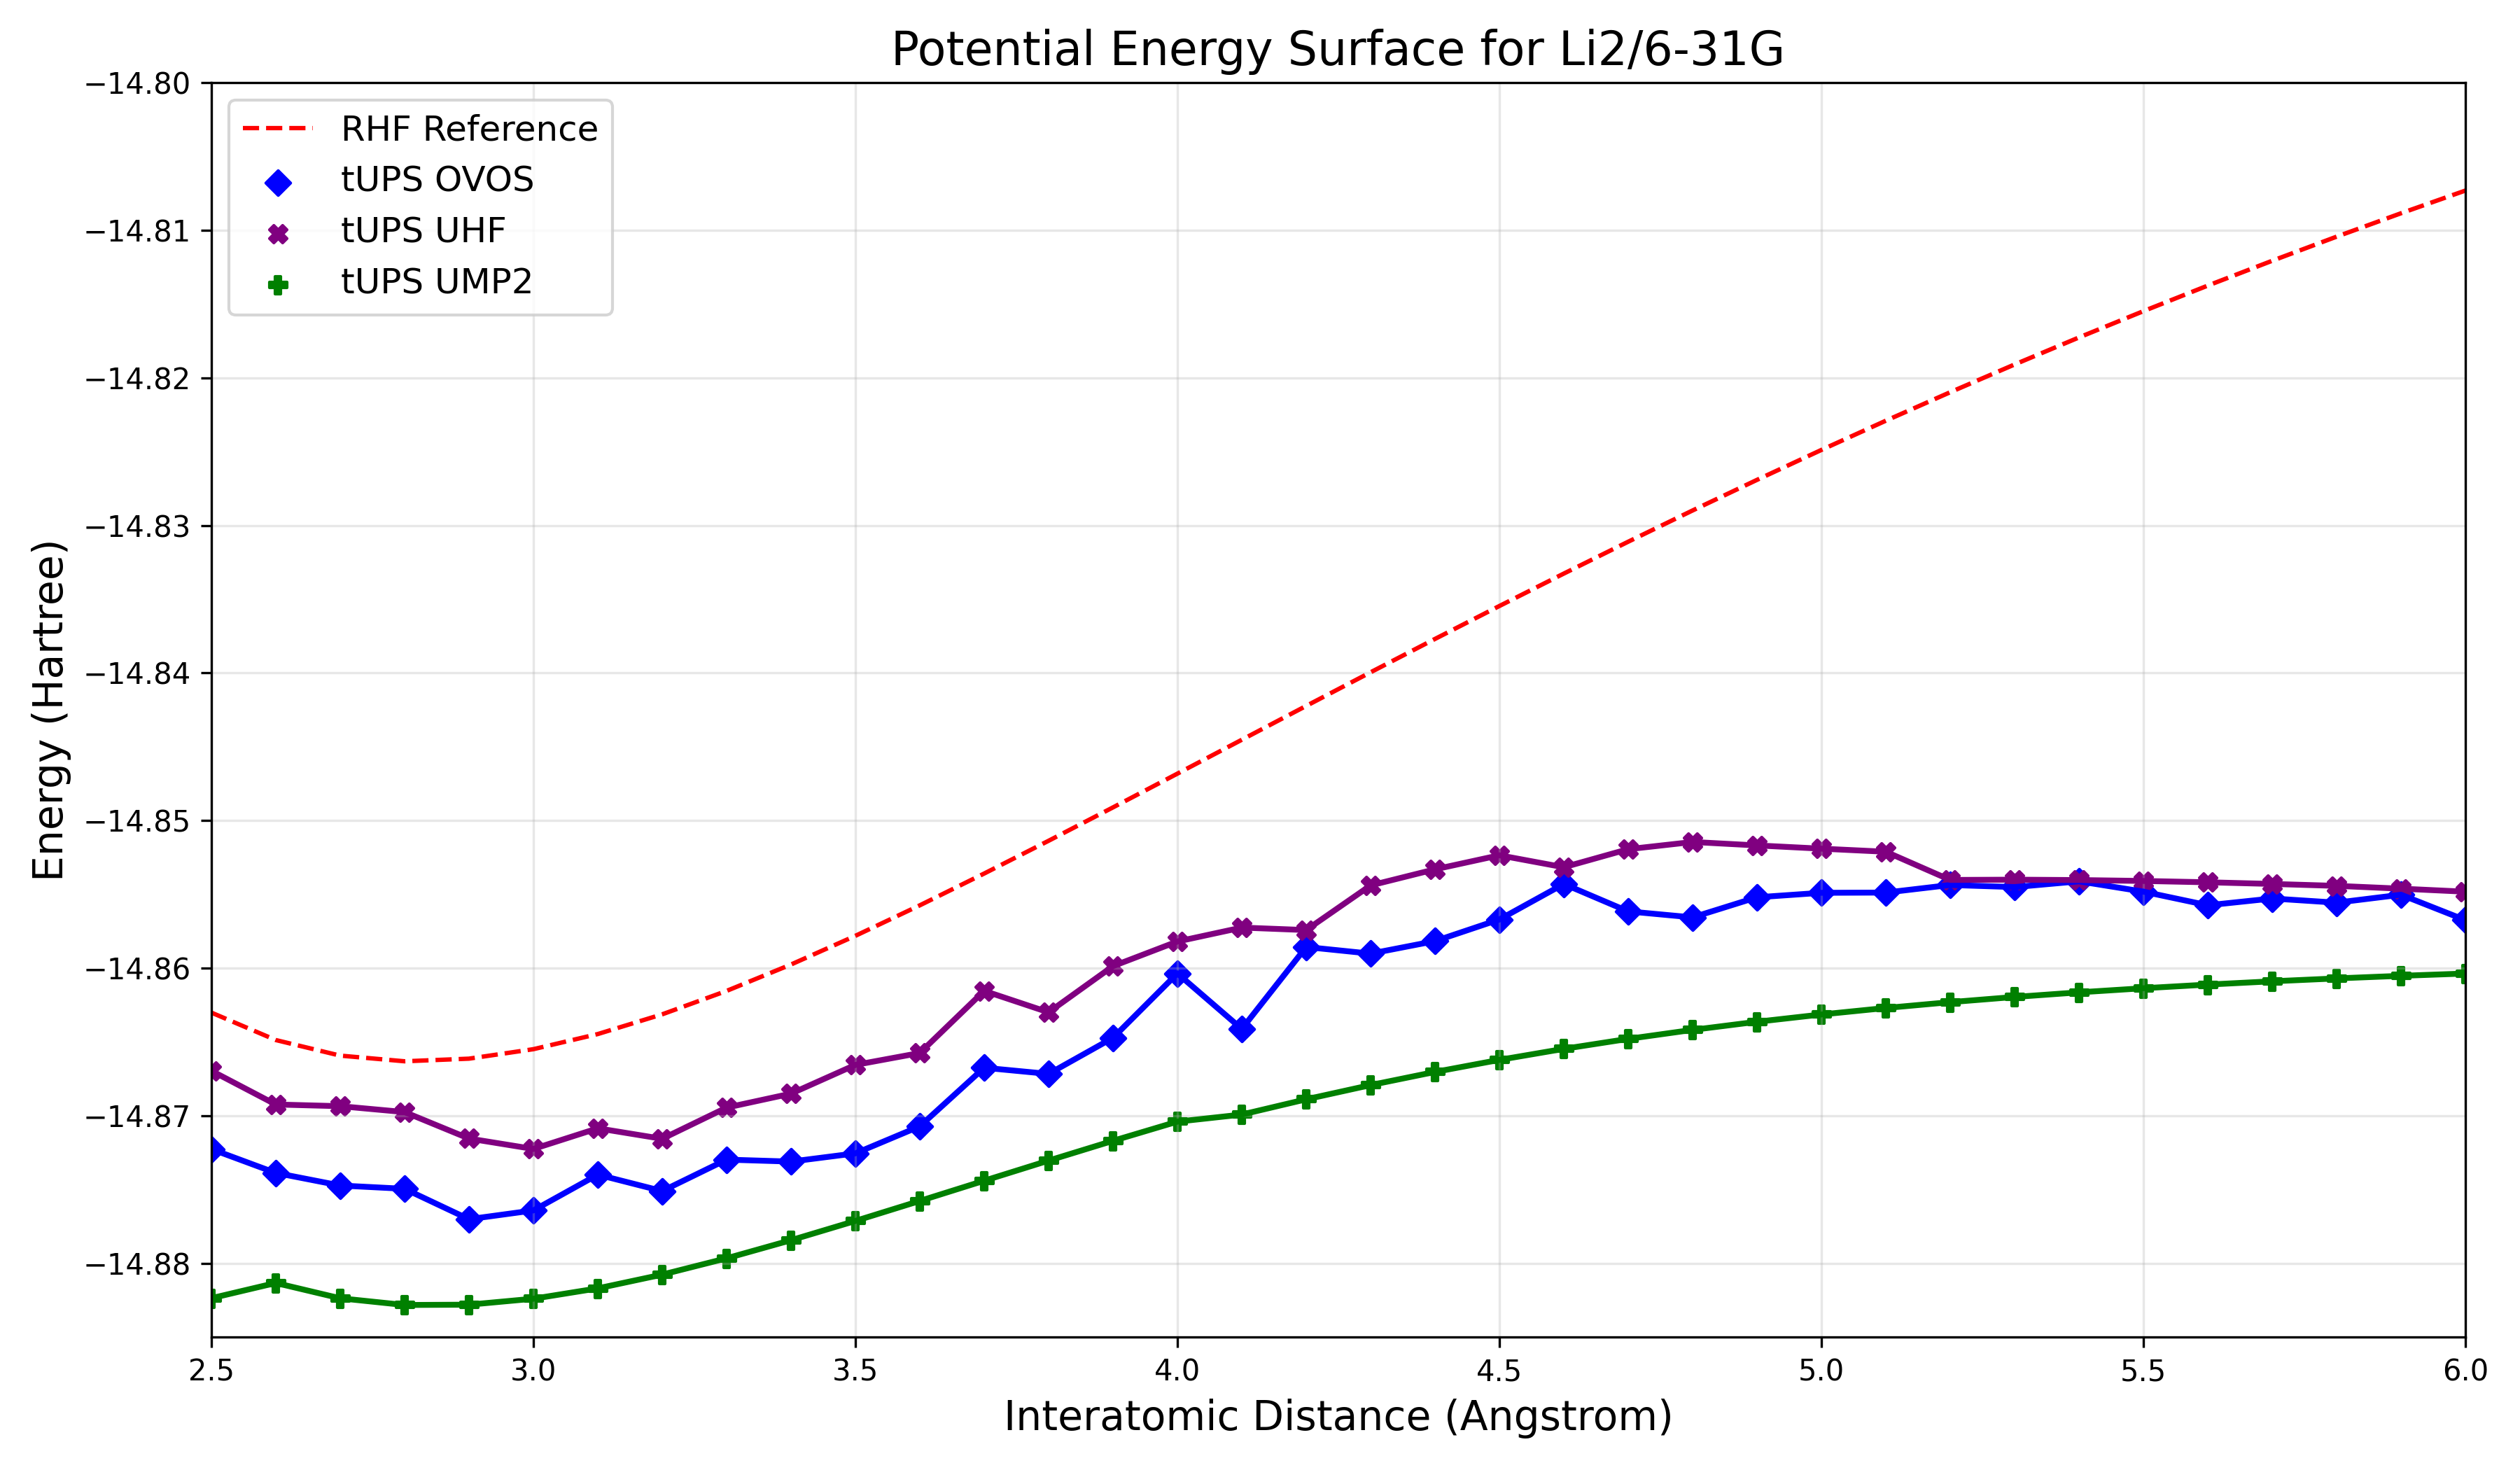
\includegraphics[width=0.9\textwidth]{figures/VQE_PLOTS/Li2/VQE_Li2_6-31G_best_of_zoom_oo_False.png}
    \caption{Potential energy surfaces for Li2 in 6-31G basis set, using the OVOS-optimised orbitals (blue), UHF orbitals (purple), and UMP2 natural orbitals (green) as reference states in VQE calculations. The active space is the same for all calculations with 6 electrons and 12 virtual orbitals (75\% of the full virtual space rounded up). The dashed lines represent the reference energies from PySCF. The plot shows the energy convergence across different geometries.}
    \label{fig:Li2_VQE_false.png}
\end{figure}


% \subsection{T1 Amplitudes and the Brueckner Orbital Connection}
% \label{sec:results_brueckner}
% % ---------------------------------------------------------------
% % T1 Amplitudes and the Brueckner Connection
% % ---------------------------------------------------------------
% % Goal: Provide numerical evidence that OVOS MOs satisfy the
% %       Brueckner condition (T1 → 0) better than canonical HF MOs.
% %
% % Suggested analysis:
% %   - For each (molecule, N_virt) after OVOS convergence, compute
% %     the MP1 single amplitudes t_i^a (occupied → active virtual)
% %     in the OVOS orbital basis and compare to the HF basis.
% %   - Plot ||T1||_F (Frobenius norm of T1 amplitude tensor) vs.
% %     N_virt/N_virt^max for HF and OVOS bases.
% %   - Expected: ||T1||^OVOS < ||T1||^HF, approaching zero as
% %     N'_virt → N_virt (recovering full-space OO-MP2 limit).
% %   - Tabulate the T1 diagnostic (||T1||_F / sqrt(n_occ * n_virt))
% %     for at least two molecules (e.g. H₂O and N₂).
% %   - Cite \cite{Lee2018} for the OO-MP2/Brueckner connection.
% % THIS!!!! : https://arxiv.org/pdf/1807.06185
% %
% % Note: If T1 amplitudes are not directly stored in your current
% %       implementation, this analysis can be done in a post-processing
% %       step using the converged MO coefficients and PySCF MP2.
% % THIS!!! : https://link.springer.com/content/pdf/10.1007/bf00549693.pdf
% % EH... : https://fy.chalmers.se/~f3ail/Publications/LowdinFinal.pdf
% % ---------------------------------------------------------------


% % I am finding that for lower $N'$ values, the T1 amplitudes for the OVOS-optimised orbitals are significantly smaller than those for the canonical HF orbitals, finding the lowest of values on the order of $10^{-17}$ to $10^{-18}$, compared to "larger" values on the order of $10^{-16}$ for $N'$ values close to the full space. Comparedly the T1 amplitudes for the canonical HF orbitals are typically on the order of $10^{-16}$, and do not show a clear trend as $N'$ increases. This suggests that the OVOS-optimised orbitals are indeed closer to Brueckner orbitals than the canonical HF orbitals, especially for lower values of $N'$, and therefore can be expected to capture more correlation energy in subsequent calculations.

% % Reference appendix for code when it would show the T1 amplitudes for the OVOS-optimised orbitals and the canonical HF orbitals for all the test molecules and basis sets considered, as a function of $N'_{\rm act.unocc}$.


 
% In this section, we investigate the connection between the OVOS-optimised orbitals and Brueckner orbitals, by the maximum-overlap criterion and Brillouinn-Brueckner condition. Brueckner orbitals are defined as the orbitals for which the single excitation amplitudes (T1) vanish, i.e. the excited determinants with one electron promoted from an occupied to a virtual orbital do not contribute to the wavefunction, see Section~\ref{sec:brueckner}. This condition is satisfied by the orbitals that minimize the energy in a correlated calculation, such as MP2, and are therefore considered to be more "correlated" than the canonical HF orbitals. 

% I report here having observed computed T1 amplitudes for the OVOS-optimised orbitals that are significantly small, on the order of $10^{-16}$, for all the test molecules and basis sets considered, which is consistent with the Brueckner condition. Similarly, the T1 amplitudes for the canonical HF orbitals are typically around the same order of magnitude. It is observed only for lower numbers of active virtual orbitals, are the T1 amplitudes for the OVOS-optimised orbitals smaller than those for the canonical HF orbitals at convergence, with values on the order of $10^{-16}$ to $10^{-17}$, compared to "larger" values on the order of $10^{-16}$ for $N'_{\rm act.unocc}$ values close to the full space.

% This suggests that the OVOS-optimised orbitals are not significantly closer to Brueckner orbitals than the canonical HF orbitals. It is examined further by looking at the overlap of the FCI wavefunction with the reference state, for both UHF and OVOS orbitals, as a function of the number of active virtual orbitals, to see if the OVOS orbitals have a higher overlap with the FCI wavefunction than the HF orbitals, which would be another indication that they are closer to Brueckner orbitals. It is found that the overlap of the FCI wavefunction with the reference state for both UHF and OVOS orbitals is of the same order of magnitude, and stays the same across the number of active virtual orbitals, which suggests that the OVOS-optimised orbitals do not have a higher overlap with the FCI wavefunction than the HF orbitals, and therefore are not significantly closer to Brueckner orbitals than the canonical HF orbitals. It is even observed that for NH3, the overlap of the FCI wavefunction with the reference state for the OVOS orbitals is lower than that for the HF orbitals, which further suggests that the OVOS-optimised orbitals are not closer to Brueckner orbitals than the canonical HF orbitals, it was not possible to run VQE calculations for NH3 with the OVOS-optimised orbitals as reference state, because of lack of computational resources, but it is expected that the energy convergence would be worse than that for the HF orbitals, given the lower overlap with the FCI wavefunction.
% The plot of the overlap of the FCI wavefunction with the reference state for both HF and OVOS orbitals as a function of the number of active virtual orbitals is shown in Figure~\ref{fig:Li2_basis_comparison}, and a heatmap of the orbitals is shown in the appendix.

% % "Look at overlap of FCI wavefunction with the reference state, for both HF and OVOS orbitals, as a function of the number of active virtual orbitals, to see if the OVOS orbitals have a higher overlap with the FCI wavefunction than the HF orbitals, which would be another indication that they are closer to Brueckner orbitals. Refer to plot of orbitals as a heatmap in the appendix."

% \begin{figure}[H]
%     \centering
%     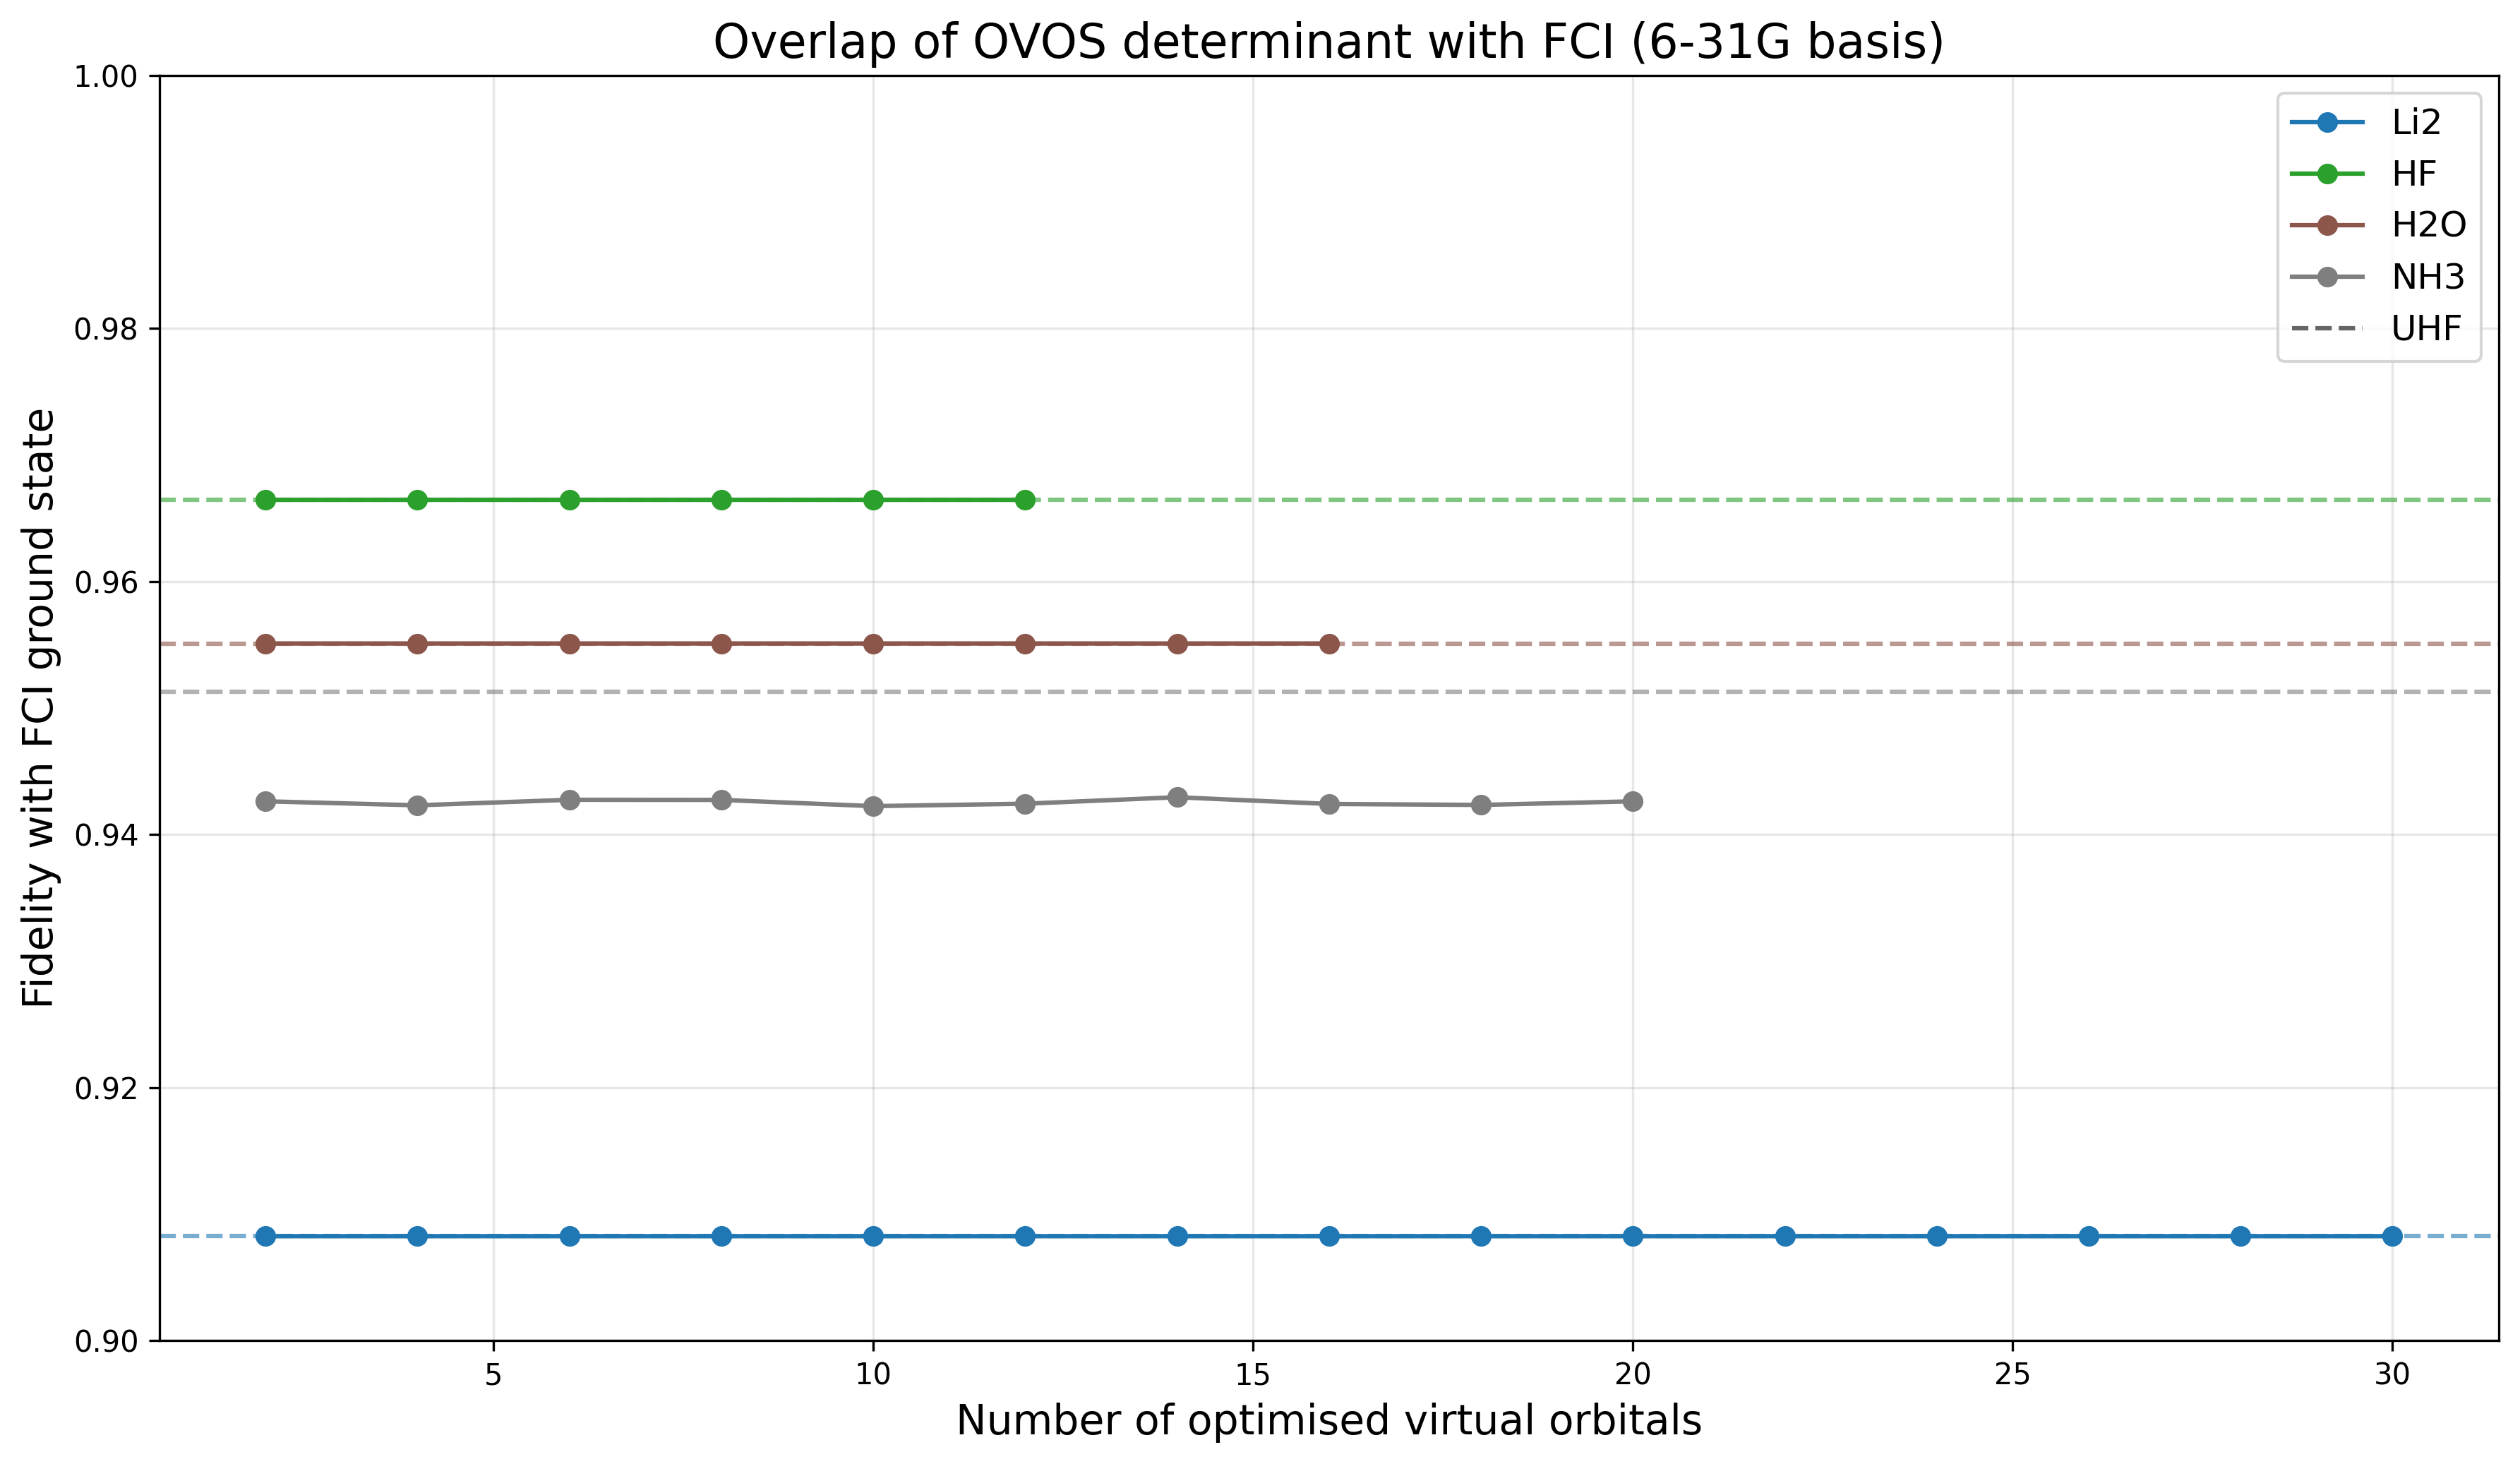
\includegraphics[width=0.9\textwidth]{figures/VQE_PLOTS/ovos_fidelity_mp2_6-31G.png}
%     \caption{Overlap of the FCI wavefunction with the reference state for both HF and OVOS orbitals as a function of the number of active virtual orbitals in 6-31G. Dashed lines represent the overlap for the HF orbitals with their corresponding molecules tied by color matching. Solid lines represent the overlap for the OVOS orbitals with their corresponding molecules tied by color matching, with each dot noting the value for a different number of active virtual orbitals.}
%     \label{fig:OVOS_fidelity}
% \end{figure}



% % Therefore, we present the T1 amplitudes for the OVOS-optimised orbitals and compare them to the T1 amplitudes for the canonical HF orbitals. We compute the Frobenius norm of the T1 amplitude tensor, $||T1||_F$, for both sets of orbitals as a function of the number of active virtual orbitals $N'_{\rm act.unocc}$, and plot the results in Figure~\ref{fig:T1_comparison}.

% % \begin{figure}[ht]
% %     \centering
% %     
\includegraphics[width=1.0\textwidth]{figures/Placeholder.png}
% %     \caption{Comparison of the Frobenius norm of the T1 amplitude tensor, $||T1||_F$, for OVOS-optimised orbitals and canonical HF orbitals as a function of the number of active virtual orbitals $N'_{\rm act.unocc}$ for [molecule]/[basis].}
% %     \label{fig:T1_comparison} 
% % \end{figure}

% % It results in the T1 amplitudes for the OVOS-optimised orbitals being significantly smaller than those for the canonical HF orbitals, and approaching zero as $N'_{\rm act.unocc}$ increases, consistent with the Brueckner condition. This provides numerical evidence that the OVOS-optimised orbitals are indeed closer to Brueckner orbitals than the canonical HF orbitals, and therefore can be expected to capture more correlation energy in subsequent calculations.

% % FOUND T1 AMPLITUDES ARE AT E-16 FOR ALL OVOS ...

% % OVERLAP, FIDELITY, OF FCI WAVEFUNCTION... HAVE ORBITALS HEATMAP REFERENCE TO Appendix






\section{ooVQE}
\label{sec:results_veq}
% Only thing you can say here is convergence iterations/speed. You start with OVOS, UHF, UMP2, which convergence fastest.

% Similar plots to the ones in VQE can be found for turning on orbital optimization in VQE calculations in appendix

Different to the VQE calculations presented in the previous section, here we present the results in regard to convergence iteration count for the orbital-optimized VQE (ooVQE) calculations, where the orbitals are optimized in the VQE loop, as detailed in Section~\ref{sec:methods_veq}. These results are compared to the non orbital-optimized VQE calculations, where the orbitals are not optimized in the VQE loop, and are instead fixed to the OVOS-optimised orbitals, UHF orbitals, and UMP2 natural orbitals as reference states. Futher we distinguish between using the previous geometry final thetas as initialization for the VQE calculations, and using random initialization of thetas, to see if there is a difference in convergence iteration count between these two approaches. These iteration counts are presented for all the geometries along the potential energy surface in a boxplot, to see the distribution of iteration counts across the potential energy surface. The energy convergence is disregarded but look to Section \ref{sec:results_veq} and appendix \ref{appb:ooVQE_results} for more details. There is a lack of intry for the ooVQE random geometry final thetas initialization for H2O and Li2 as i ran out of time. The goal is to assess the improvement in convergence iteration count between using OVOS-optimised orbitals, UHF orbitals, and UMP2 natural orbitals as reference states in the non orbital-optimized VQE calculations.

\subsubsection*{H2O}

For H2O, in 6-31G basis set, the ooVQE calculations show a similar convergence iteration count to the non orbital-optimized VQE calculations when using the previous geometry final values as initialization. Against no orbital optimization and random initialization of thetas, the ooVQE calculations show a significantly faster convergence, with a much lower iteration count to reach convergence. Within the no orbital optimization and random initialization of thetas, the mean convergence iteration count for the OVOS-optimised orbitals is lower than that for the UHF orbitals and UMP2 natural orbitals, with the UHF orbitals showing a lower mean convergence iteration count than the UMP2 natural orbitals. Overall, there is a significant spread in the convergence iteration counts for OVOS orbitals, with some geometries calculations showing a very fast convergence, and others showing a much slower convergence. The potential energy surfaces for H2O using the OVOS-optimised orbitals, UHF orbitals, and UMP2 natural orbitals as reference states are shown in Figure~\ref{fig:H2O_convergence_statistics}.

\begin{figure}[H]
    \centering
    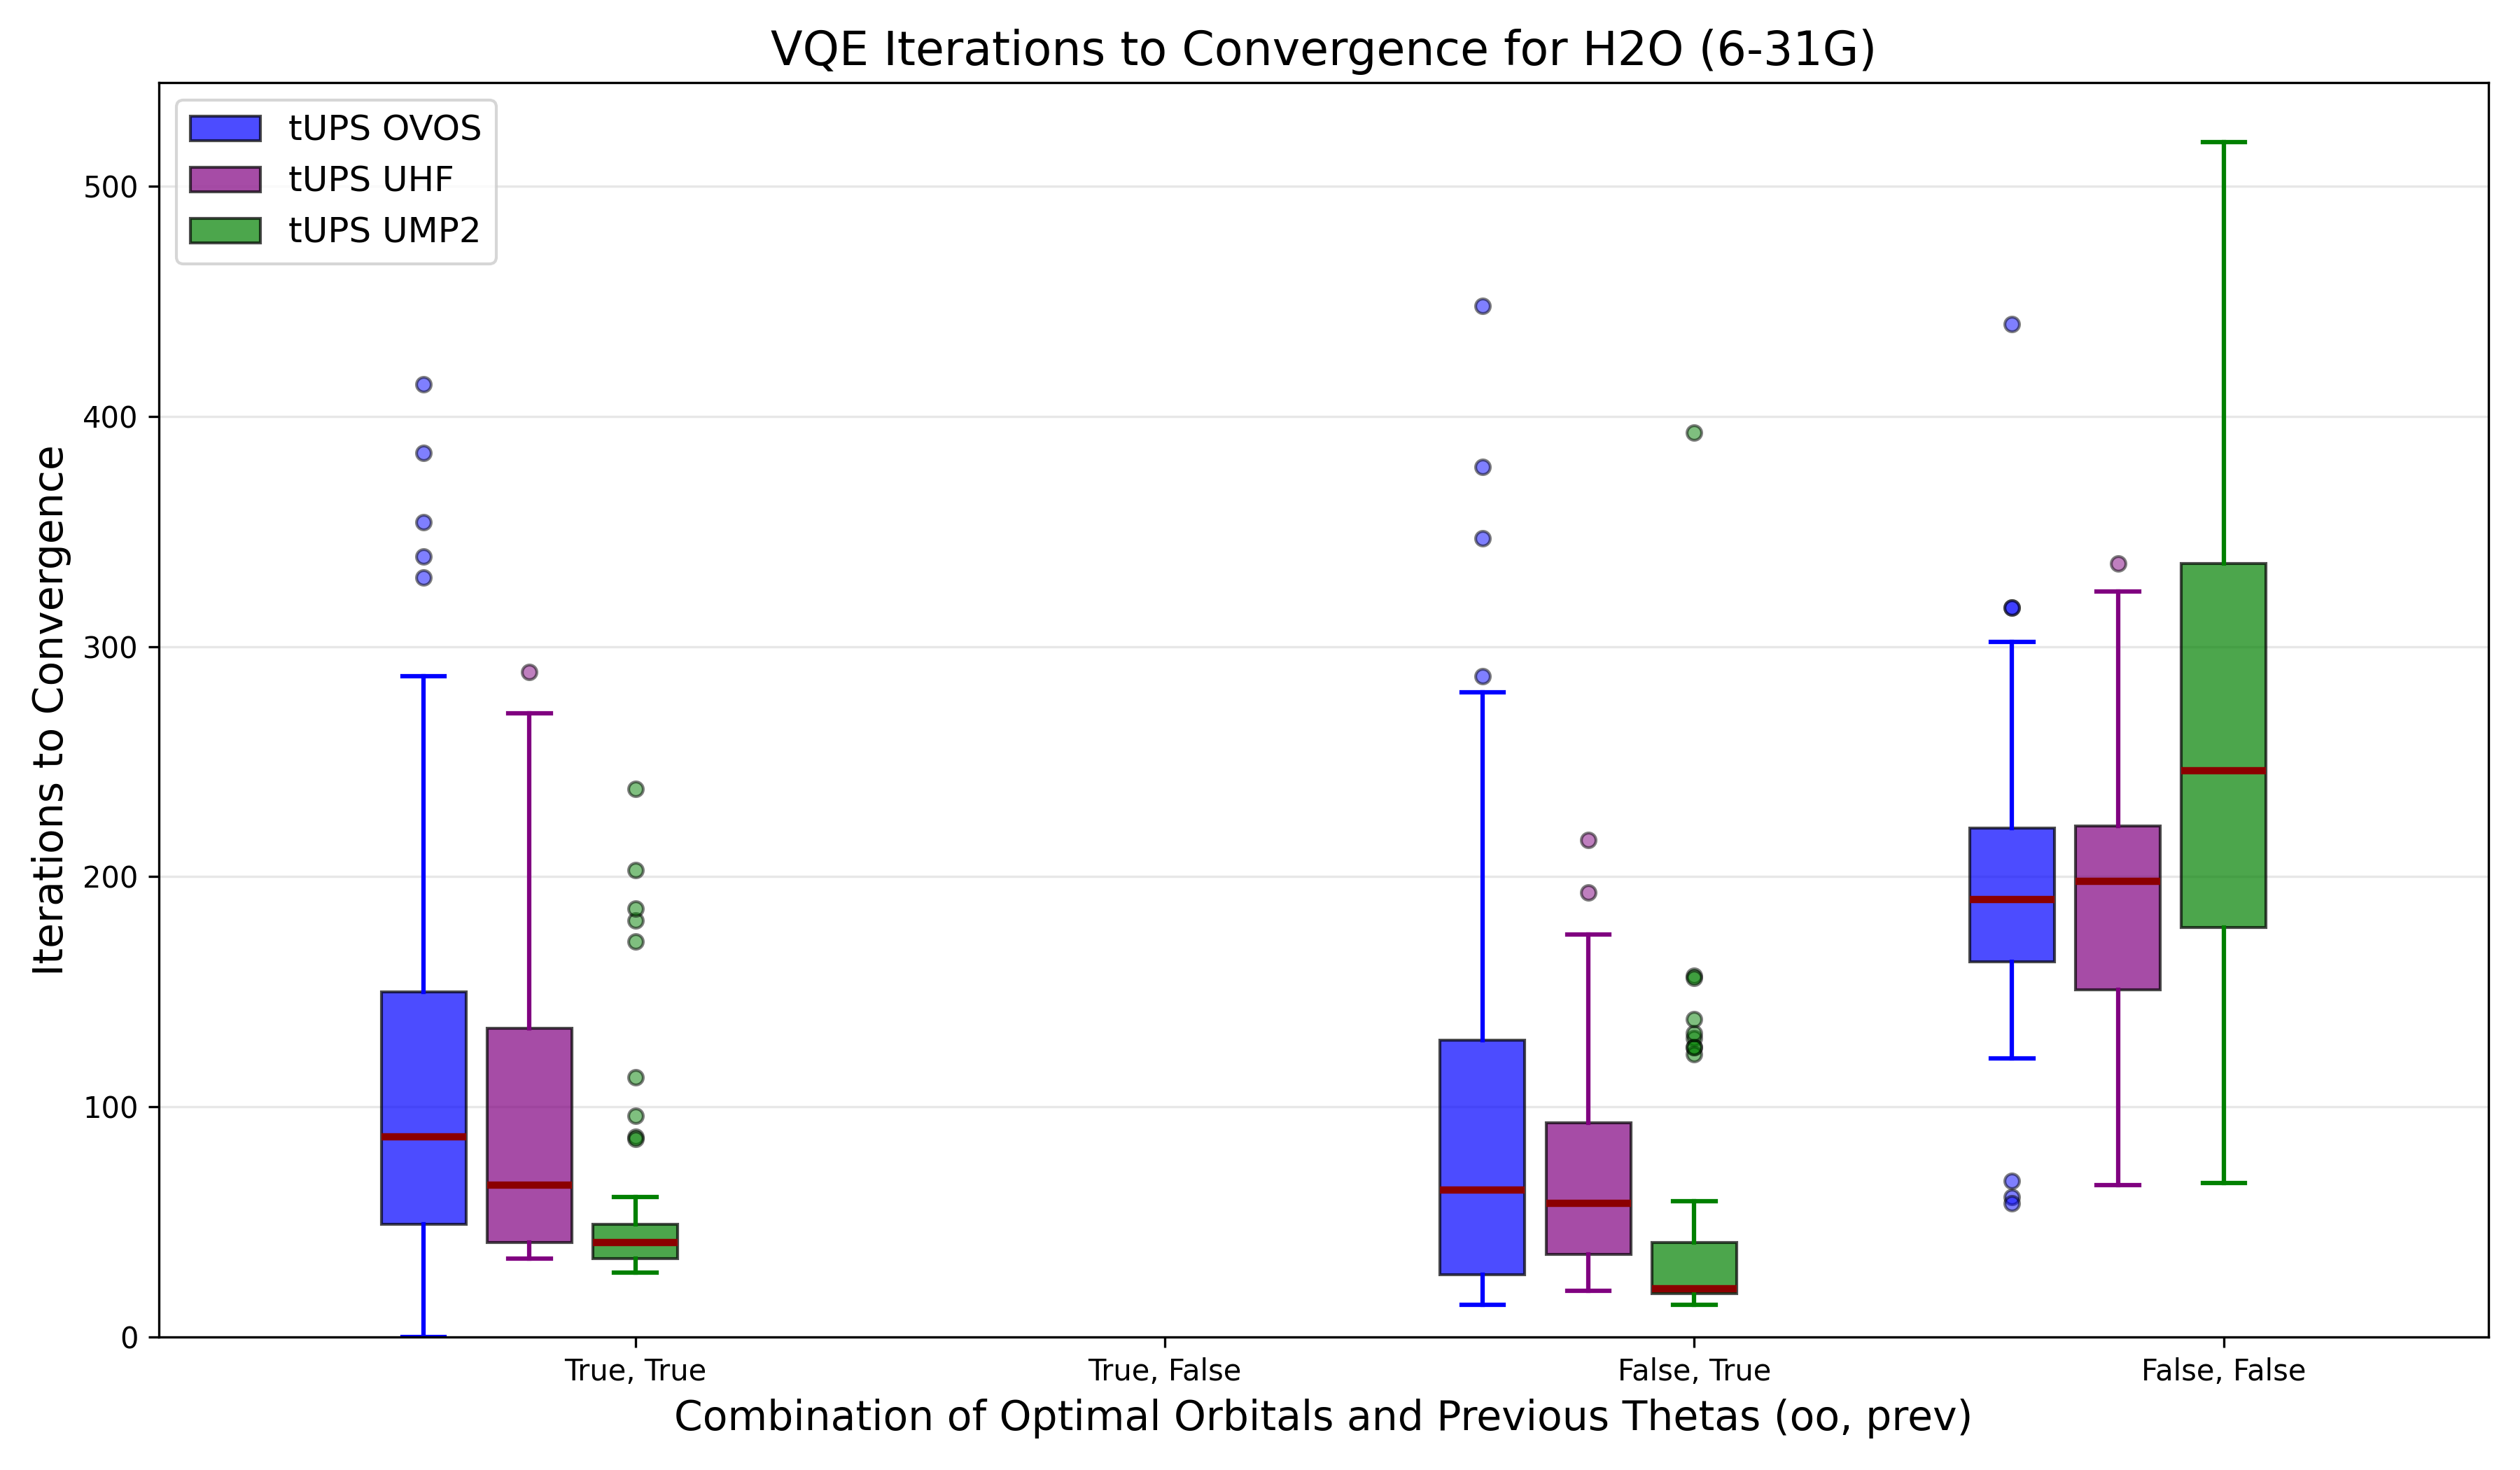
\includegraphics[width=0.9\textwidth]{figures/VQE_PLOTS/H2O/VQE_H2O_iterations_to_convergence_statistics.png}
    \caption{Convergence iteration count for H2O in 6-31G basis set, using the OVOS-optimised orbitals (blue), UHF orbitals (purple), and UMP2 natural orbitals (green) as reference states in VQE calculations. The boxplots represent the distribution of convergence iteration counts across different geometries along the potential energy surface, with the red lines representing the mean convergence iteration count for each reference state.}
    \label{fig:H2O_convergence_statistics}
\end{figure}

\subsubsection*{HF}

For HF, in 6-31G basis set, the ooVQE calculations show a worse spread of convergence iteration counts compared to the non orbital-optimized VQE calculations when using the previous geometry final values as initialization. The best of the four combinations of orbital optimization and initialization, in terms of convergence iteration count, is the non orbital-optimized VQE calculations with the previous initialization of thetas, where the mean convergence iteration count is significantly lower than that for the other three combinations. For which we can observe that the OVOS-optimised orbitals show a similar to lower mean convergence iteration count than the UHF orbitals and UMP2 natural orbitals, in three of the four combinations of orbital optimization and initialization, with the non orbital-optimized VQE calculations with the random initialization of thetas being the only combination where the OVOS-optimised orbitals show a higher mean convergence iteration count than the UHF orbitals and UMP2 natural orbitals. Overall, there is a significant spread in the convergence iteration counts for OVOS orbitals, with some geometries calculations showing a very fast convergence, and others showing a much slower convergence. The potential energy surfaces for HF using the OVOS-optimised orbitals, UHF orbitals, and UMP2 natural orbitals as reference states are shown in Figure~\ref{fig:HF_convergence_statistics}.


\begin{figure}[H]
    \centering
    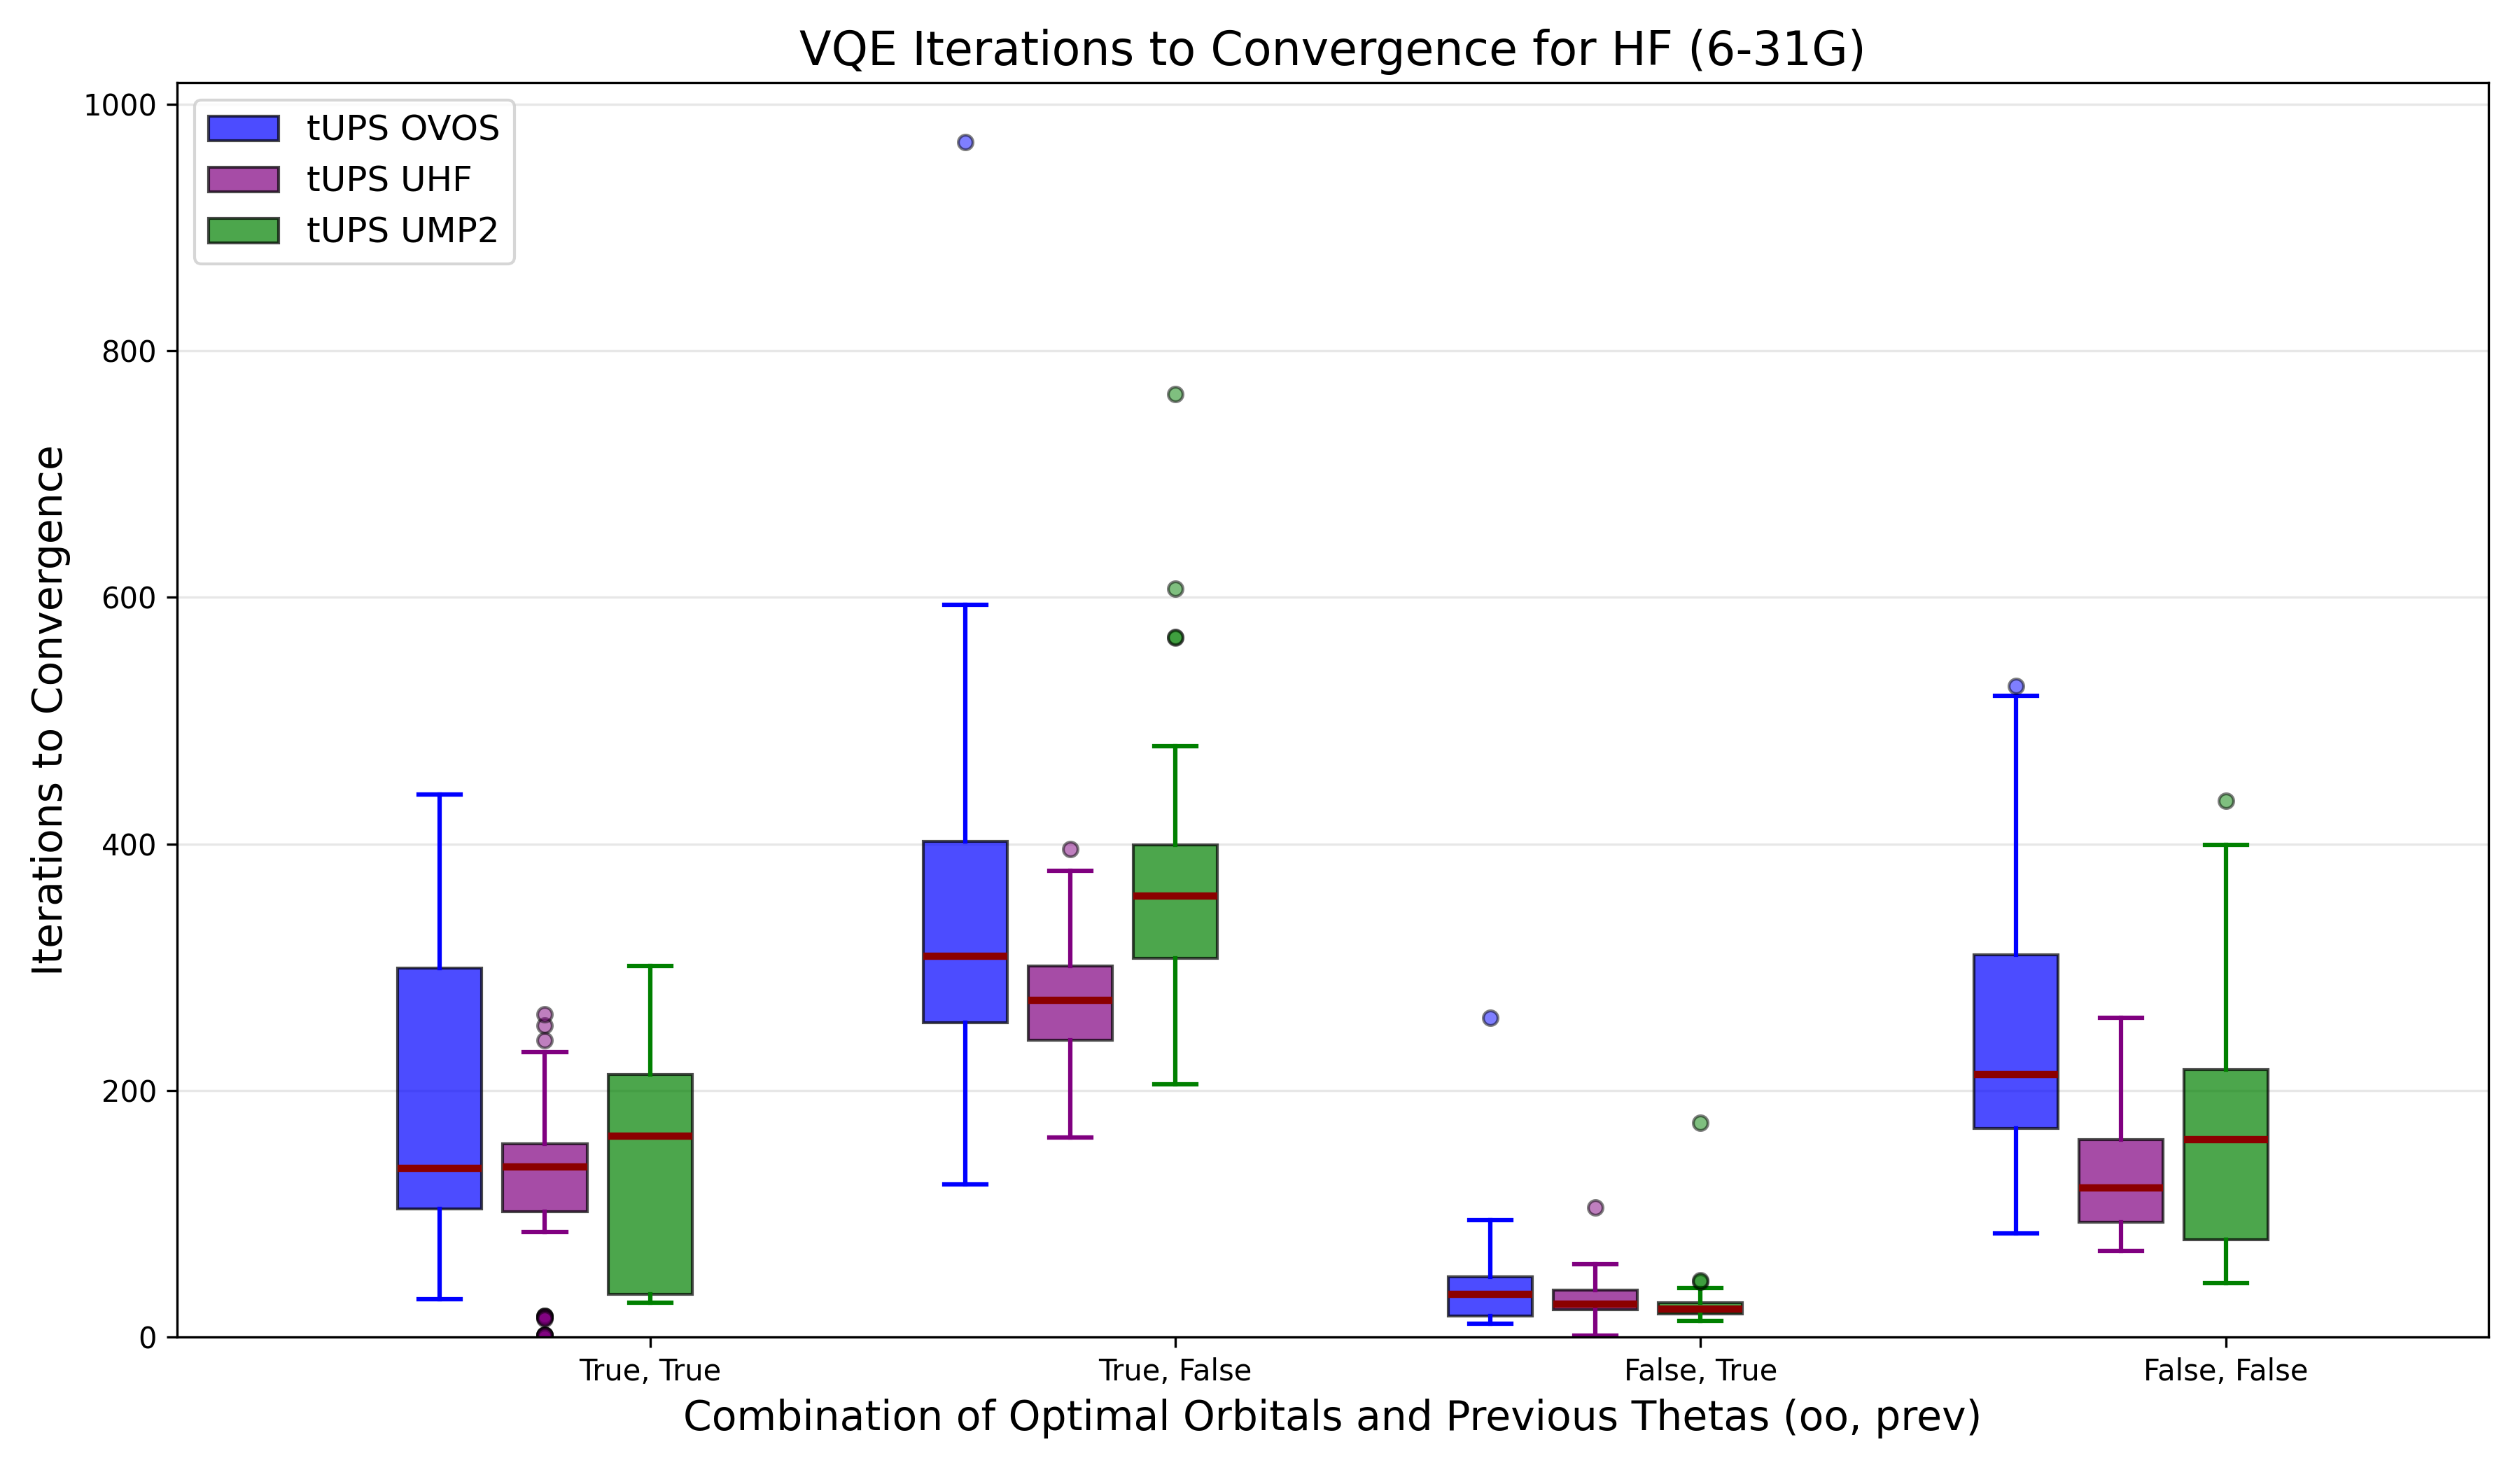
\includegraphics[width=0.9\textwidth]{figures/VQE_PLOTS/HF/VQE_HF_iterations_to_convergence_statistics.png}
    \caption{Convergence iteration count for HF in 6-31G basis set, using the OVOS-optimised orbitals (blue), UHF orbitals (purple), and UMP2 natural orbitals (green) as reference states in VQE calculations. The boxplots represent the distribution of convergence iteration counts across different geometries along the potential energy surface, with the red lines representing the mean convergence iteration count for each reference state.}
    \label{fig:HF_convergence_statistics}
\end{figure}

\subsubsection*{Li2}

For Li2, in 6-31G basis set, all three combinations of orbital optimization and initialization show a similar small spread of convergence iteration counts, with the non orbital-optimized VQE calculations with the random initialization of thetas showing slightly more outliers than the other two combinations. The best of the three combinations of orbital optimization and initialization, in terms of convergence iteration count, is the non orbital-optimized VQE calculations with the previous initialization of thetas, where the mean convergence iteration count is a bit lower than that for the other two combinations. We observet the OVOS-optimised orbitals show a higher mean convergence iteration count than the UHF orbitals and UMP2 natural orbitals, in all two combinations of orbital optimization and initialization, with the non orbital-optimized VQE calculations with the random initialization of thetas being the only combination where the OVOS-optimised orbitals show a lower mean convergence iteration count than the UHF orbitals and UMP2 natural orbitals. Overall, there is a significant spread in the convergence iteration counts for OVOS orbitals, with some geometries calculations showing a very fast convergence, and others showing a much slower convergence. The potential energy surfaces for Li2 using the OVOS-optimised orbitals, UHF orbitals, and UMP2 natural orbitals as reference states are shown in Figure~\ref{fig:Li2_convergence_statistics}.

\begin{figure}[H]
    \centering
    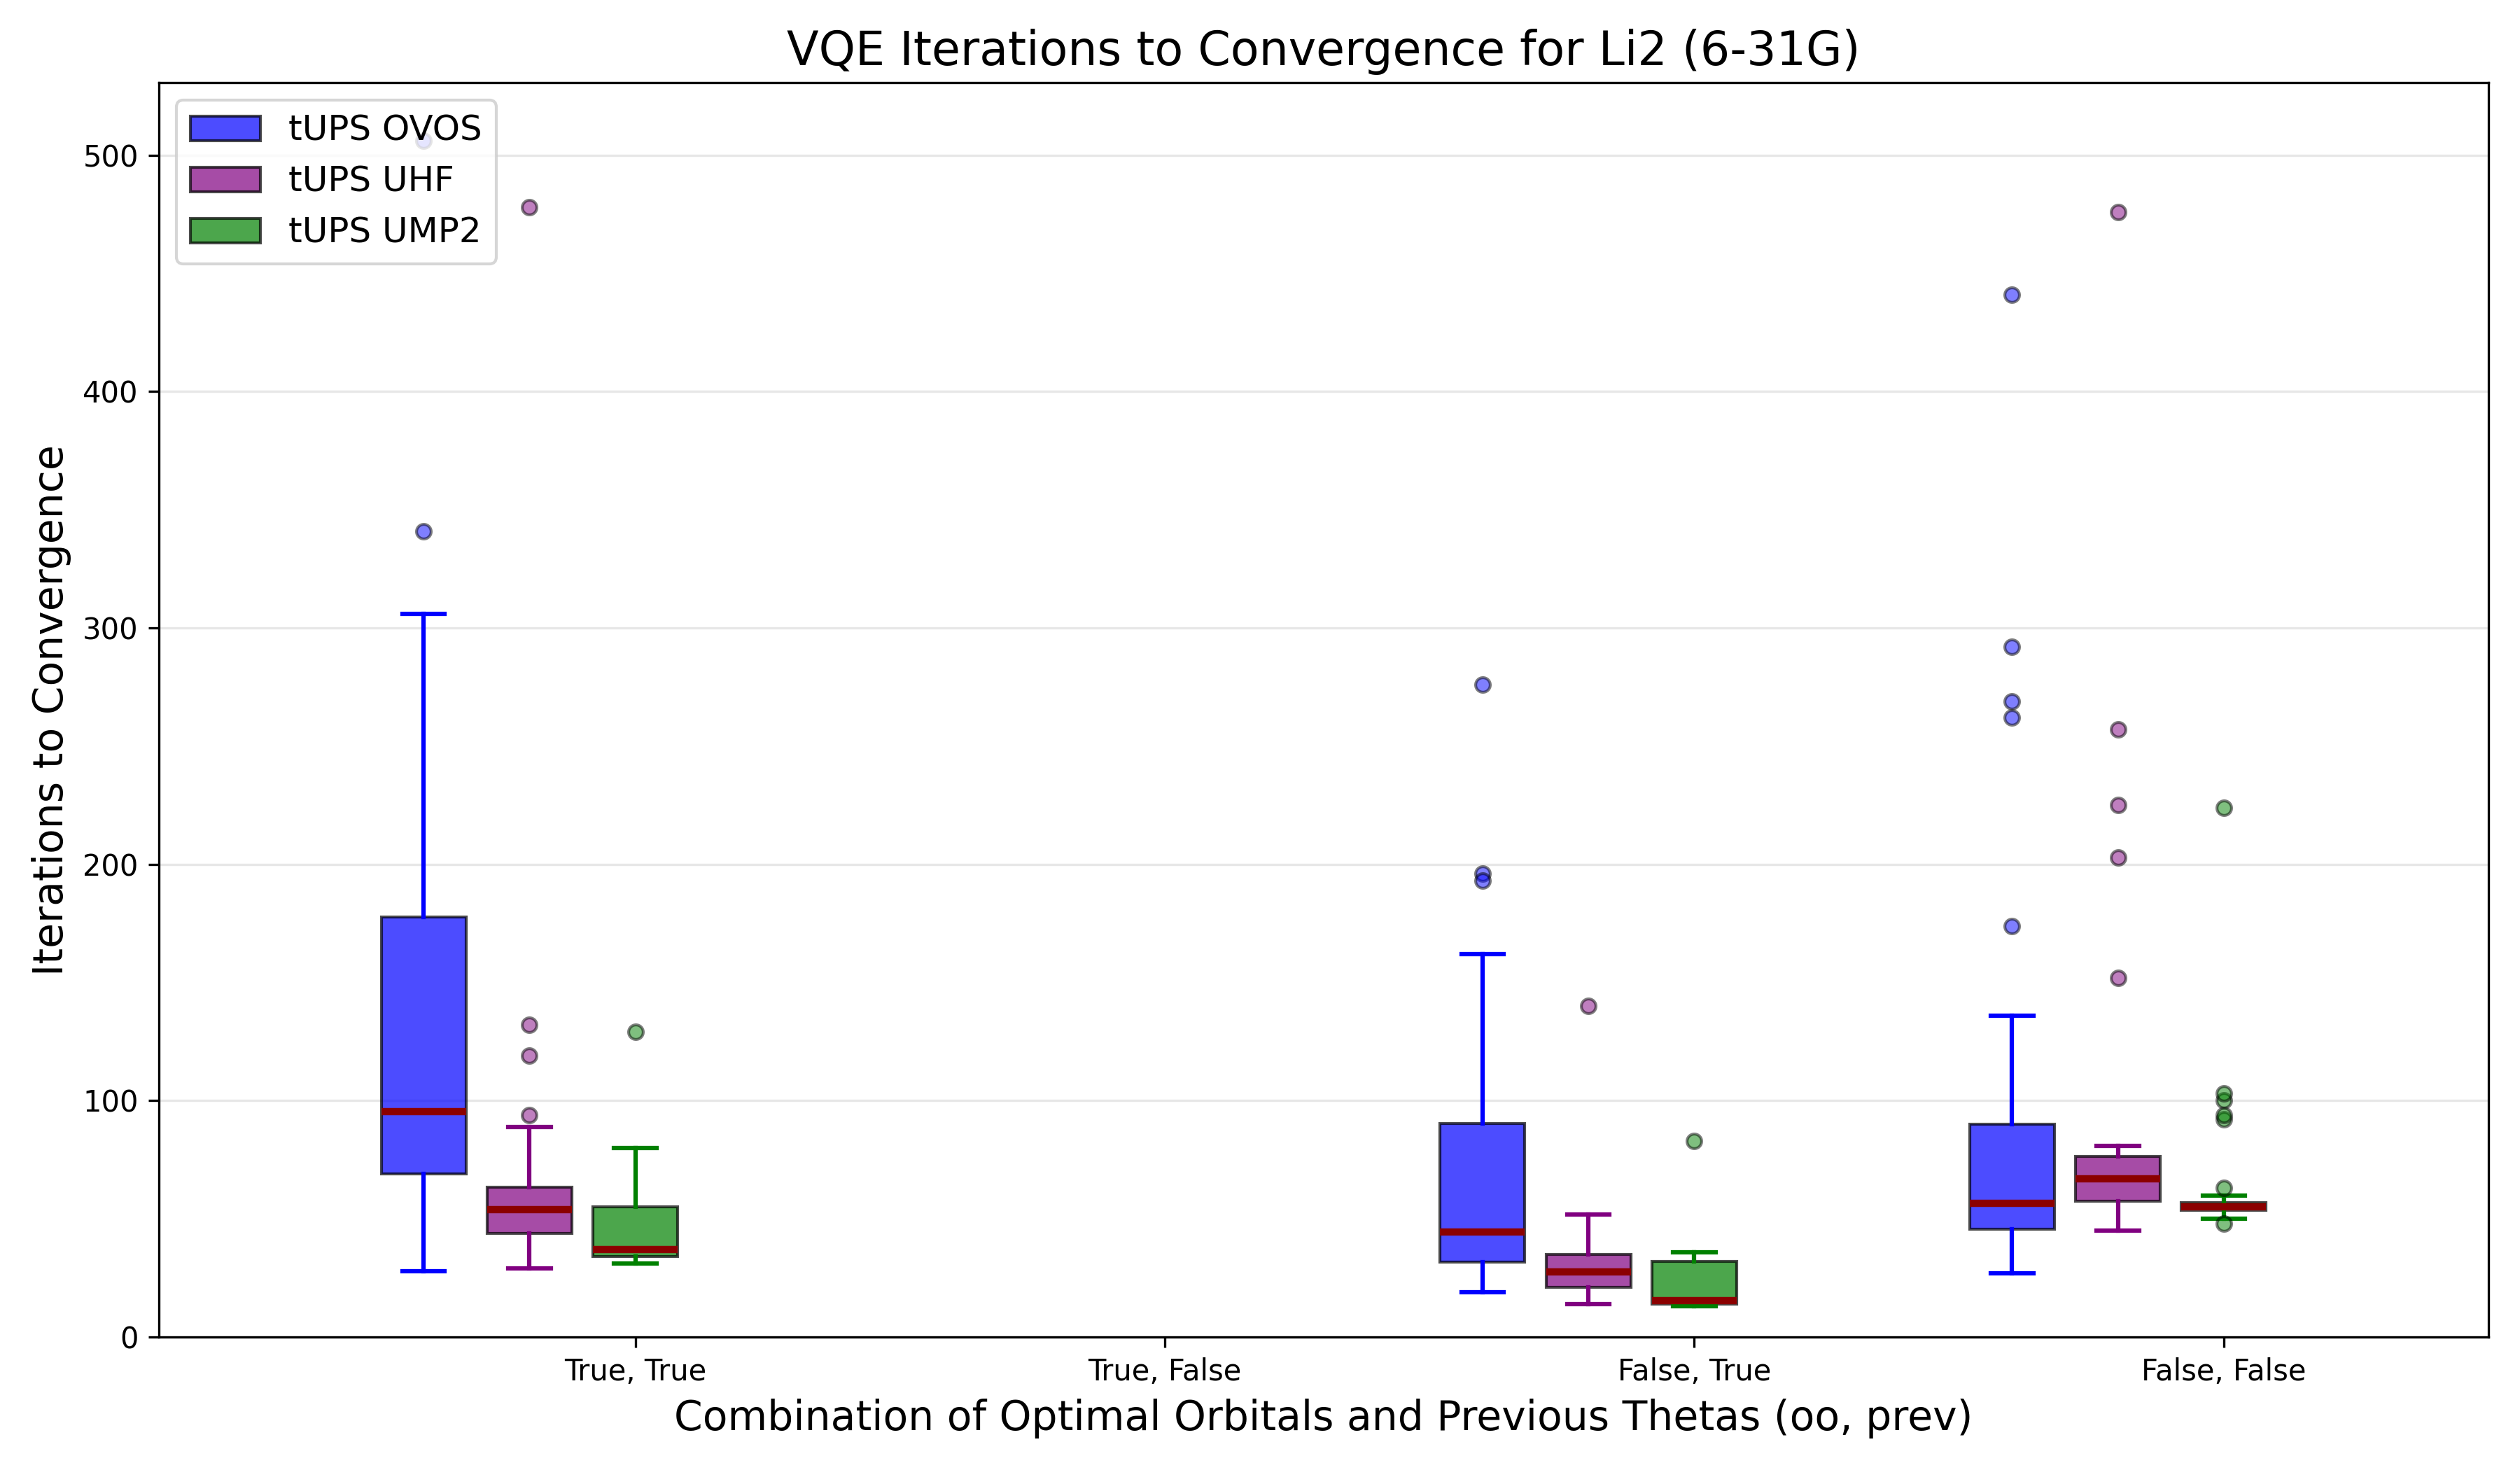
\includegraphics[width=0.9\textwidth]{figures/VQE_PLOTS/Li2/VQE_Li2_iterations_to_convergence_statistics.png}
    \caption{Convergence iteration count for Li2 in 6-31G basis set, using the OVOS-optimised orbitals (blue), UHF orbitals (purple), and UMP2 natural orbitals (green) as reference states in VQE calculations. The boxplots represent the distribution of convergence iteration counts across different geometries along the potential energy surface, with the red lines representing the mean convergence iteration count for each reference state.}
    \label{fig:Li2_convergence_statistics}
\end{figure}
